\section{Co-working}
\indent Co-working je v samotnej podstate model poskytovania obchodných služieb, ktorý zahŕňa jednotlivcov, ktorí pracujú nezávisle alebo spolupracujú v spoločných kancelárskych priestoroch. Toto zdielanie jedných priestorov umožňuje tejto skupine ľudí zdieľať hodnoty, skúsenosti, nápady a profitovať zo synergicekého efektu, ktorý prináša sústredenie talentovaných pracovníkov na jednom mieste. Tiež umožňuje spoznávanie nových ľudí, ktorí môžu byť v budúcnosti pre človeka dôležitý. Najčastejšími využívateľmi co-workingu sú napríklad obchodníci, umelci, programátori, konzultanti, dizajnéri, makléri, agenti, malé a začínajúce firmy.

\begin{figure}[H]
    \centering
    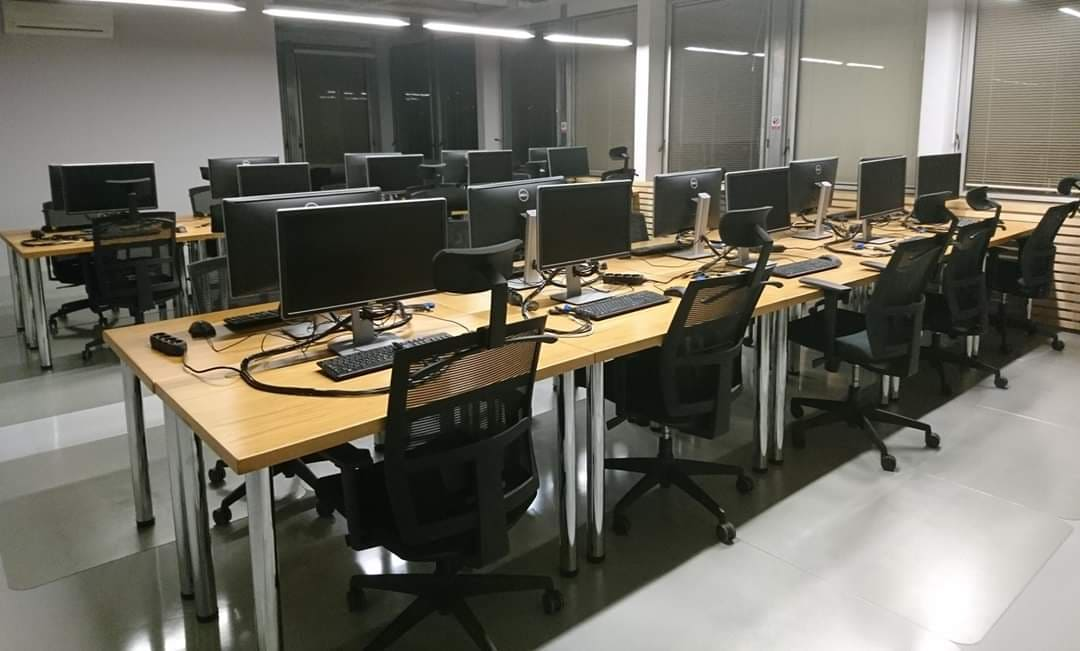
\includegraphics[scale=0.40]{img/ybase.jpg}
    \caption{Y-base študentký co-working space na internáte STU ŠD Mladosť Bratislava}
    \label{fig:img-ybase}
\end{figure}

\indent Pre účely co-workingu sa po celom svete začali budovať tzv. co-working centrá, ktorých počet každým rokom rastie. Vznik týchto centier je výsledkom hľadania stratégií, ako sa vyrovnať s rizikami a problémami nových, flexibilných štýlov práce. Veľa centier bolo založených internetovými podnikateľmi, ktorí chceli nájsť alternatívu k práci z kaviarní alebo k izolácii spôsobenej prácou z domu. Tieto centrá sú zväčša ihneď pripravené a vybavené potrebnými vecami k práci ako sú stoly, stoličky, tabuľe na písanie, kuchynka, internetové pripojenie, mítingové priestory prípadne aj sieťová tlačiareň. To znamená, že pre bežného používateľa nevyžaduje začatie práce v takomto centre žiadne počiatočné alebo investičné náklady. Jediným poplatkom je zaplatenie členstva v centre. 


\subsection{História co-workingu}
\indent Slovo coworking v zmysle popisu ľudí, ktorí pracujú v akomkoľvek prostredí prvý krát použila Bernie DeKoven v roku 1995. K prvému vzniku coworkingového priestoru respektíve centra prišlo ale až v roku 2006 v San Franciscu pod vedením Brada Neuberga. Toto centrum sa nazývalo \textit{San Francisco Coworking Space} a bolo otvorené len 2 dni v týždni. Kuriozitou je, že prvý mesiac ho nikto nevyužival lebo hoci termín coworking bol známy ale nikto ho nepočul pod významom ako coworking miesto alebo centrum. 

\begin{figure}[H]
    \centering
    
\includegraphics[scale=0.50]{img/coworking_space.jpg}
    \caption{Co-working centrum v San Franciscu}
    \label{fig:img-co-space}
\end{figure}

\indent Dnes sa vytváranie coworkingových centier pokladá za globáln fenomén, ktorý v niektorých mestách dosahuje ročný nárast až 24,2\%. Predpokladom je, že do roku 2022 bude celostvetovo vytvorených vyše 30500 centier alebo priestorov a viac ako 5,1 milióna členov. Coworking je nová cesta trvalo udržiavateľného spájanie pracovného a osobného života. Je to globálny pilier, ktorý bude formovať spôsob našej práce v budúcnosti. 

\section{Co-working aplikácie}
\indent Co-working aplikácie sú aplikácie, ktoré slúžia na komunikáciu a manažovanie tímu pri práci viac ľudí na dosiahnutie určitého cieľa alebo výsledku. Týchto aplikácii na trhu existuje veľa pričom niektoré sú bezplatné, niektoré sú platené a niektoré sú vyvinuté priamo vo firme kde sa používajú a nemá k nim teda prístup nikto okrem danej firmy. Medzi najznámejšie patrí napríklad Slack, Facebook workplace, Trello, Microsoft Teams a iné. 
\indent Tieto aplikácie majú slúžiť ako náhrada za coworkingové centrum v online svete. Keď si zoberieme služby, ktoré ponúkajú coworkingové centrá tak sa dajú prirovnať k niektorým službám, ktoré ponúkajú aplikácie. Či už sa jedná o mítingové miestosti - v aplikácii online chatové miestnosti v rámci tímu alebo o možnosť spoznávania nových ľudí osobne - v aplikácii online. 

\subsection{Slack}
\indent Slack je komunikačný nástroj vyvinutý pre pracovné využitie spoločnosťou Slack Technologies – „jedno miesto pre posielanie správ, nástroje a súbory“. To znamená, že Slack je softvér na posielanie „okamžitých“ správ s možnosťou pridania ďalších doplnkov podľa potreby používateľa. Tieto doplnky ale nie sú potrebné na plynulý chod aplikácie pretože základnou funkciou Slacku je len posielanie správ. Na Slacku existujú 2 spôsoby komunikácie: 1. spôsob sú tzv. kanály čo je v podstate skupinový rozhovor a 2. spôsob sú priame správy medzi dvoma ľuďmi. 
\subsubsection{História}
\indent Slack začal ako aplikácia na internú komunikáciu v spoločnosti Stewarda Butterfielda Tiny Speck pri vývoji online hry Glitch – hra bola vydaná v septembri 2011. Pre širšiu verejnosť bol Slack vydaný v auguste 2013. Slack je skratka pre: „Searchable Log of All Conversation and Knowledge“ čo vo voľnom preklade znamená „Protokol prehľadávania všetkých konverzácií a znalostí.“

\indent V marci 2015 spoločnosť Slack oznámila, že bola vo februári 2015 napadaná hackermi počas 4 dní. Počas tohto útoku boli ohrozené údaje používateľov. Medzi tieto údaje patrili e-mailové adresy, používateľské mená, heslá, telefónne čísla a Skype mená ktoré boli priradené k ich účtom. Po tomto útoku Slack pridal do svojej aplikácie dvojfaktorovú autentifikáciu. 
\subsubsection{Používateľské rozhranie}
\indent Keď chce používateľ začať používať Slack musí najskôr cez stránku Slacku vytvoriť názov svojej „inštancie“ Slacku. Tento názov sa potom stane súčasťou URL adresy, ktorá slúži ako pozvánka. Potom buď cez stránku Slacku alebo poslaním URL pozve ľudí, ktorých chce mať na svojom Slacku. 

\indent Po akceptovaní tejto pozvánky si používateľ vytvorí účet. Po prihlásení pod týmto účtom sa používateľovi otvorí stránka „inštancie“ Slacku alebo ak má nainštalovanú aplikáciu tak aplikácia Slacku viď. Obr.~\ref{fig:img-slack-app}

\indent Kanály na Slacku môžu byť verejné čo znamená, že každý člen skupiny ho vidí a môže sa k nemu pripojiť alebo súkromné čo znamená, že ich vidia len ľudia pridaný alebo pozvaný. Priame správy sú vždy súkromné ale môžu obsahovať až 8 ľudí.

\begin{figure}[H]
    \centering
    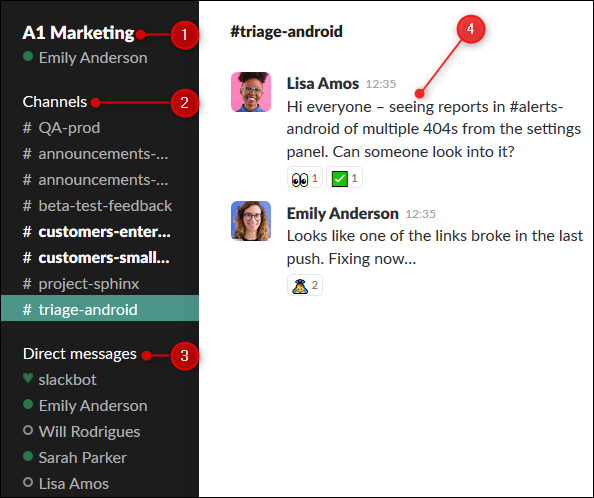
\includegraphics[scale=0.80]{img/obr1.png}
    \caption{Slack aplikácia}
    \label{fig:img-slack-app}
\end{figure}
\begin{enumerate}
    \centering
    \item Názov skupiny/inštancie
    \item Zoznam kanálov 
    \item Zoznam kontaktov
    \item Okno chatu
\end{enumerate}


\subsubsection{Doplnky}
\indent Do aplikácie Slack je možné pridať rôzne doplnky či už priamo vytvorené firmou Slack Technologies alebo inými firmami ako je Google, Jira, Trello a iné. Celkový prehľad doplnkov Slack uvádza na svojej stránke kde sa vie používateľ priamo prekliknúť aj na stránku daného doplnku kde je napísané čo doplnok prináša do Slacku plus tutoriál ako ho používať prípadne video používania doplnku. Doplnok je možné pridať priamo cez aplikácie Slack alebo cez stránku Slacku.

\indent Doplnky sú na stránke rozdelené do kategórii, do ktorých viac menej patria. Tieto kategórie sú rôzne od botov, ktorý automaticky ako je niečo zmenené na strane doplnkovej aplikácie, pridajú do daného kanála upozornenie alebo správu, až po priame importy, ktoré pridávajú funkcionalitu priamo do Slacku.
\subsubsection{Výber najznámejších importov}
\begin{itemize}
    \item Google Drive
    \item Google kalendár
    \item Trello
    \item Twitter
    \item Outlook kalendár
    \item OneDrive
    \item GitHub
    \item Polly(hlasovania a prieskumy)
    \item Jira Cloud
    \item TimeBot
    \item WorkBot
    \item Giphy
    \item Doodle Bot
\end{itemize}
\subsubsection{Cena}
\indent Slack ako taký je zadarmo ale sú tam isté obmedzenia. Hlavným obmedzením je prístup len k 10000 najnovším správam a používateľ môže pridať len 10 doplnkov na inštanciu. Ďalšími obmedzeniami sú napríklad žiadny jedno-kanálový alebo viac-kanálový hostia a limitované možnosti administrácie. 

\indent Ak chce používateľ sprístupniť celú funkcionalitu je to dosť drahé. Vychádza to približne 12 dolárov na používateľa mesačne pri ročnej platbe alebo približne 15 pri mesačnej platbe. Ak teda napríklad máme 1000 člennú skupinu, ktorá chce používať Slack vychádza to približne 144000 dolárov pri ročnej platbe.

\subsection{Facebook Workplace}
\indent Čas, ktorý ľudia strávili v práci chatovaním, prezeraním a likovaním príspevkov na Facebooku znižoval produktivitu ľudí cca v hodnote 3,5 bilióna dolárov. Táto téma sa pretriasala cez seriózne diskusie až po vytváranie vtipných obrázkov. Preto sa ľudia vo Facebooku začali zaoberať touto otázkou či sa funkcionalita Facebooku nedá preniesť aj na pracovnú aplikáciu. Toto dalo počiatok Facebook Workplacu, ktorý podľa slov jeho stvoriteľov má podporiť kolaboráciu tým, že ju urobí zábavnou a jednoduchšou pre ľudí.

\begin{figure}[H]
    \centering
    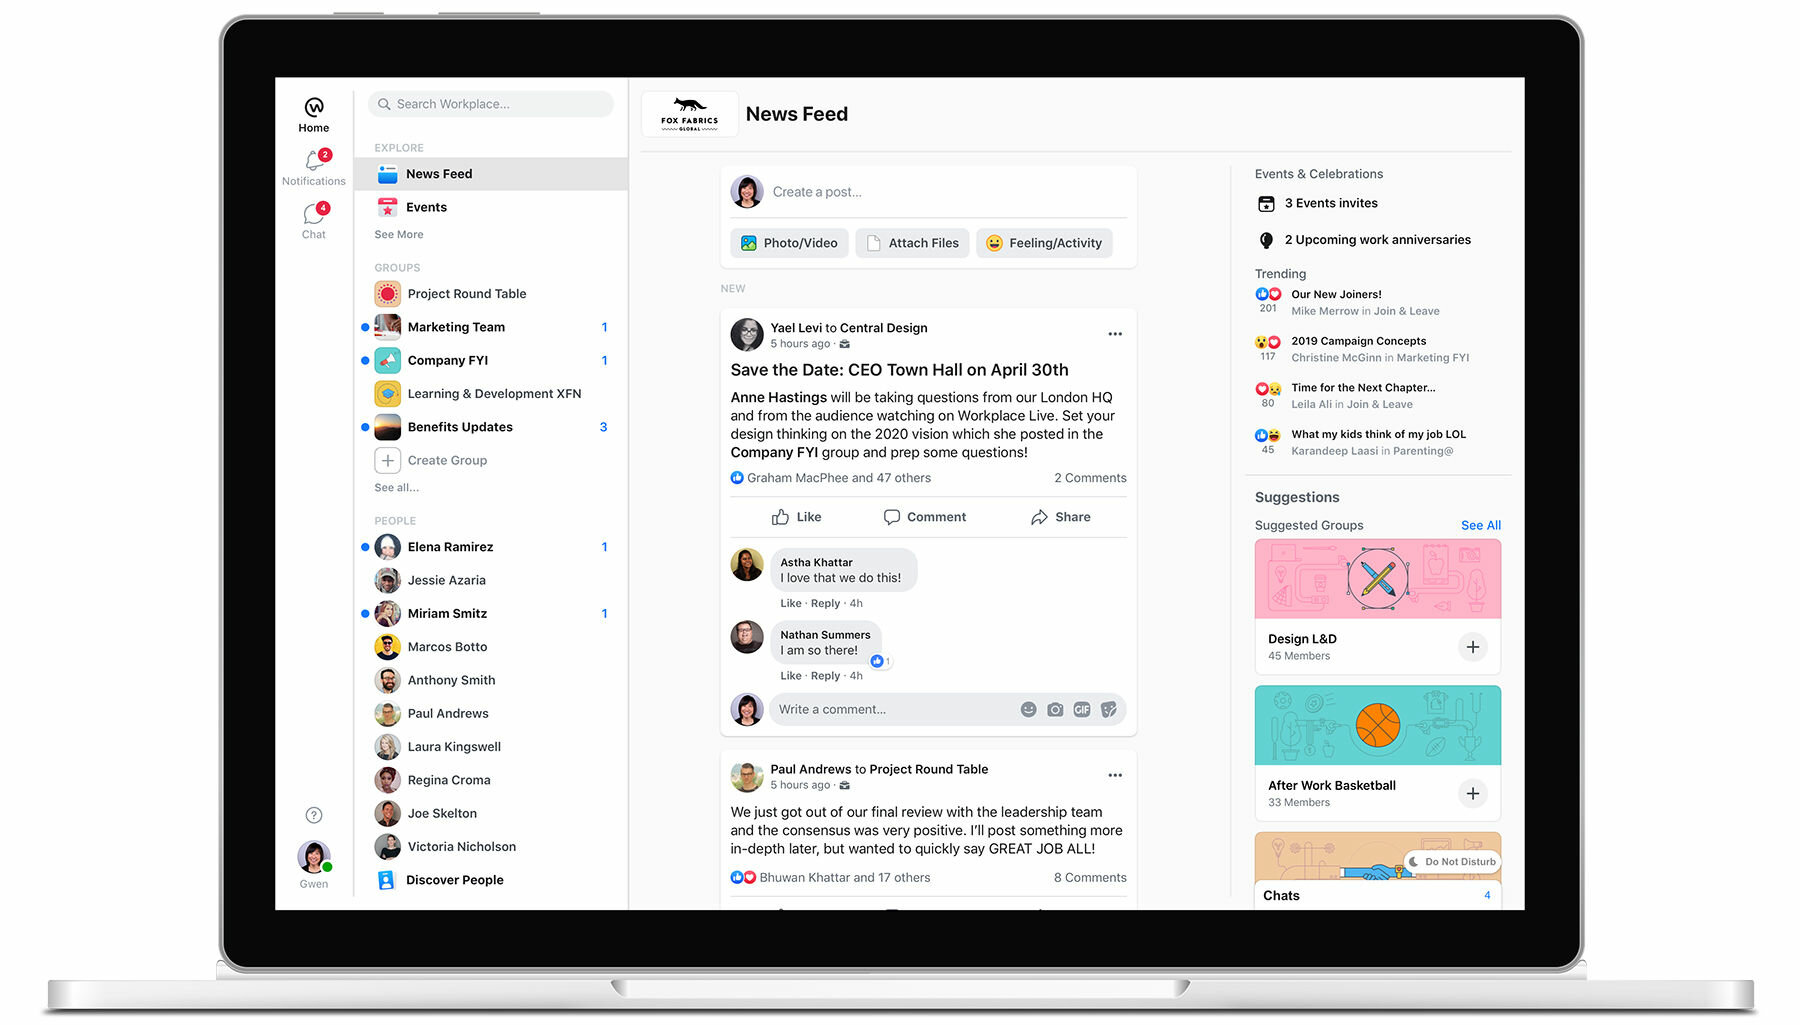
\includegraphics[scale=0.25]{img/obr-fb-workplace.jpg}
    \caption{Stránka Facebook Workplace}
    \label{fig:img-fb-workplace}
\end{figure}

\subsubsection{História}
\indent Myšlienka sa začala rozvíjať v roku 2014 keď prišla myšlienka nasmerovať tendenciu členov tímu prechádzať Facebook počas pracovnej doby k lepšej produktivite a spolupráci. Začiatkom roku 2015 sa začala do vybraných spoločností zavádzať beta verzia s názvom Facebook at Work. Keďže Facebook týmto vstupoval do neznámych vôd bolo samozrejmé, že beta verzia sa veľmi často menila. V polovici roka 2015 Facebook získal veľmi silného spojenca pre vývoj tejto aplikácie - The Royal Bank of Scotland – Škótska národná banka. Tá u seba presadila masívne využitie tejto beta verzie Facebook at Work kedy sa vytvorilo až 100000 nových účtov. 

\indent Ku koncu roka 2015 mal Facebook veľa kladných ohlasov na túto svoju vyvíjanú platformu od manažérov firiem kde bol Facebook at Work zavedený. Bolo to hlavne zapríčinené tím, že zamestnanci mali veľmi jednoduchý prístup k pracovným profilom svojich kolegov a podriadených. Tak isto kvôli prehľadnosti sa názov zmenil na Facebook Workplace.

\indent  V októbri 2016 boli oficiálne na trh uvedené pracovné a mobilné verzie aplikácie Facebook Workplace. Týmto Facebook začal konkurovať gigantom ako Slack a Microsoft Teams (vtedy Skype for Business) na poli podnikového softvéru.
\subsubsection{Používateľské rozhranie}
\indent Rozhranie Workplacu je podľa slov používateľov na 95\% rovnaké ako to na Facebooku. Väčšina populárnych funkcii Facebooku bola pridaná tiež do Workplacu:
\begin{itemize}
    \item Newsfeed – zobrazujú sa tu všetky tímové aktivity ako napríklad príspevky členov tímu, firemné akcie a všetky informácie týkajúce sa práce prihláseného používateľa
    \item Live tools – funkcie na živý prenos (Live streaming)
    \item Skupiny – manažéri môžu vytvárať skupiny na pracovisku a tým udržiavať aktivity jednotlivých skupín/tímov na jednom  mieste
    \item Správy – používatelia si môžu písať so svojimi kolegami
\end{itemize}

\indent Pre používateľov je toto síce výhoda keďže sa nemuseli učiť používať nový nástroj avšak pre firmy je problém prijať v podstate napodobeninu Facebooku ako pracovnú aplikáciu. Kvôli tomuto Facebook aj oddelil profily Facebooku a Workplacu nakoľko do nedávna boli tieto profily prepojené a aj vytváranie účtu sa robilo cez profil Facebooku. 
\subsubsection{Cena}
\indent Workplace je pre firmy na prvé tri mesiace zadarmo. Potom sa jeho cena odvíja od počtu aktívnych účtov. Do 1000 používateľov sa platia 3 doláre za každého, do 10000 používateľov sa platí 2 doláre za každého a nad 10000 používateľov sa platí 1 dolár za každého.  Pre neziskové organizácie a akademické účely je úplne zadarmo aj po 3 mesiacoch.

\subsection{Microsoft Teams}
\indent Microsoft Teams je aplikácia na pracovnú komunikáciu a kolaboráciu od spoločnosti Microsoft, ktorá bola vyvinutá aby konkurovala aplikáciám Slack, Workplace, HipChat. Vo svojej najjednoduchšej podobe je to aplikácia umožňujúca komunikáciu medzi členmi vytvorenej skupiny na báze miestností - kanálov. Microsoft sa už pred vydaním Teams pokúšal presadiť na trhu pracovných aplikáciu pomocou svojho Skype for Business. Táto aplikácia avšak nenaplnila očakávania tak ako jej lepšia verzia Teams. 
\subsubsection{História}
\indent V marci 2016 chcel Microsoft kúpiť Slack za 8 miliárd dolárov avšak Bill Gates bol proti a skôr presadzoval zlepšenie ich aplikácie Skype for Business. Tento nákup presadzoval hlavne vysoko postavený pracovník Microsoftu Qi Lu. Ten avšak ešte v roku 2016 opustil spoločnosť a v Novembri toho istého roku Microsoft oznámil prácu na aplikácii Teams ako na aplikácii, ktorá má konkurovať Slacku. 

\indent Slack uznal Teams ako konkurenčnú službu avšak uviedol, že nekonkurujú rovnakému publiku nakoľko Teams v tej dobe neumožňoval ľudom bez predplateného balíka Office 365 vstup do aplikácie Teams. Slack to zdôvodňoval aj tým, že neprepokladá sa, že by malé a stredné podniky, ktoré už Slack používajú nezačnú používať platenú službu Office, ktorej Teams bol súčasťou. Neskôr však Teams pridal možnosť pridania nových ľudí aj bez predplateného balíka Office 365. Slack na toto reagoval integráciou služieb od Google (Drive, Kalendár, Gmail). 

\indent V roku 2017 sa udiali 2 udalosti. Prvou bolo, že Teams nahradili MS Classroom v balíku Office 365 for Education. Druhou udalosťou bola správa v septembri, že Teams nahradzujú Skype for Business. Tým bola aj ukončená služba Skype for Business. 

\begin{figure}[H]
    \centering
    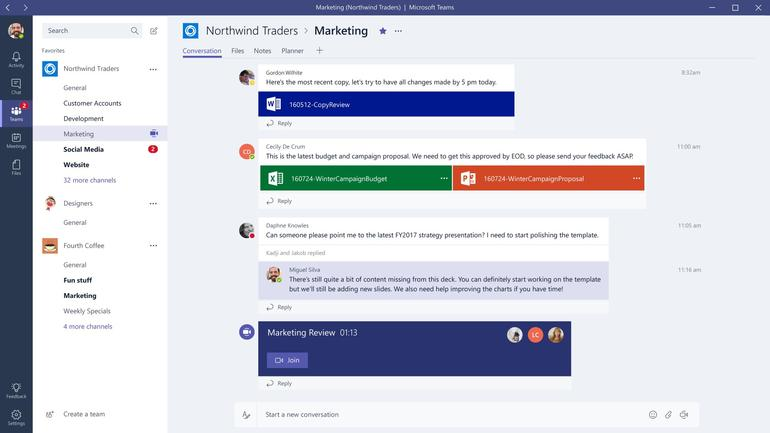
\includegraphics[scale=0.70]{img/obr-ms-teams.jpg}
    \caption{Aplikácia MS Teams}
    \label{fig:img-ms-teams}
\end{figure}

\indent V júli 2018 oznámil Microsoft bezplatnú verziu služby Teams s obmedzeniami typu počet používateľov a kapacitu ukladania súborov. V novembri 2019 dosiahol Teams 20 miliónov používateľov čo bol nárast o 7 miliónov od júla 2019. 
\subsubsection{Používateľské rozhranie}
\indent Rozhranie Teams je veľmi podobné tomu na Slacku. Na vytvorenie tímu treba vytvoriť URL, ktorá potom slúži rovnako ako na Slacku na pozívanie používateľov. Po prihlásení sa pomocou Microsoft účtu potom môžu už jednotlivý používatelia vytvárať miestnosti, do ktorých môžu pridávať príspevky. Tak isto je možná komunikácia medzi používateľmi bez miestnosti štýlom ako je v aplikácii Skype. Tu je povolená aj hlasová a video komunikácia Skype štýlom. 

\indent Mimo klasických miestností-kanálov je možne vytváranie aj takzvaných meeting miestností, ktoré slúžia na komunikáciu počas pracovných porád, meetingov a stretnutí. Tieto miestnosti umožňujú priame pridanie času a dátumu meetingu do kalendára Outlooku Náhľad nástenkya po otvorení miestnosti je možné vidieť v akom stave stretnutie je: ešte nezačalo, prebieha, ukončené. 

\indent Microsoft do Teams pridal aj funkciu podobnú funkcionalite Trella – dashboard. Pomocou tejto funkcie môžu manažéri, učitelia, vedúci prideľovať a sledovať prácu používateľov. Tak isto sa jednotlivé úlohy na tejto „nástenke úloh“ dajú komentovať, presúvať alebo hodnotiť.

\indent Samozrejmosťou je veľmi dobrá kompatibilita s inými aplikáciami Microsoftu ako je Word, Excel, PowerPoint, OneDrive. Jednotlivé dokumenty týchto aplikácii sa dajú priamo posielať, upravovať v aplikácii Teams a tak majú jednotlivý používatelia vždy najaktuálnejšiu verziu dokumentu k dispozícii. Microsoft pridal ale aj komunikáciu s aplikáciami od iných vývojárov ako je GitHub, Evernote, Zendesk pomocou konektorov. Táto komunikácia slúži najmä na posielanie upozornení, že na strane druhej aplikácii prišlo k nejakej zmene – napríklad príde upozornenie do miestnosti, že niektorý používateľ pushol na git niečo nové.  
\subsubsection{Doplnky}
\indent Do Teams podobne ako do Slacku je možne pridanie rôznych doplnkov od iných vývojárov. Tieto doplnky sú avšak po väčšine len Boti, ktorých úlohou je posielanie upozornení, že na strane druhej aplikácie prišlo k nejakej zmene – pridanie nových vecí na github, zmena v Evernote a iné. Týchto Botov je potvrdených zatiaľ 85 a 70 konektorov – aplikácie, ktoré slúžia nielen na posielanie upozornení. 
\subsubsection{Cena}
\indent Microsoft Teams je v svojej jednoduchšej podobe zadarmo. Obmedzeniami bezplatnej verzie sú napríklad prístup na OneDrive, plánovania schôdze, nahrávanie schôdze pomocou Microsoft Stream, technická podpora, viacfaktorová autentifikácia pre všetkých používateľov. 

\indent Platených verzii je viac. Tieto verzie sú viazané na balík Office 365, ktorý má používateľ/firma zaplatený. Za balík Office 365 Business Essentials pýta Microsoft 4,20€ za používateľa mesačne s ročnou viazanosťou a za balík Office 365 Business Premium 10,50€ za používateľa mesačne tak isto s viazanosťou na rok. V balíku Premium je zahrnutá všetka funkcionalita aplikácie Teams. Pri balíčku Essentials sú tam stále isté obmedzenia.

\subsection{Trello}
\indent Trello je aplikácia na vytváranie pracovnej nástenky v kanbanskom štýle. Aplikácia od roku 2017 patrí spoločnosti Atlassian avšak vydaná bola v roku 2011 spoločnosťou Fog Creek Sowtvare. Aplikácia obsahuje virtuálnu nástenku kde členovia tímu môžu vytvárať, organizovať a priraďovať úlohy v rámci projektu. Použitý kanbanský/kartový štýl umožňuje členom tímu vzájomne spolupracovať a komunikovať pri práci na projekte. Používatelia môžu k projektovým kartám pridávať komentáre, odkazy, súbory a fotografie. Trello existuje v rôznych podobách. Existuje webová aplikácia, desktopová aplikácia či už pre Windows alebo MacOS a tak isto existujú aj mobilné aplikácie pre Android a iOS. Existuje aj import aplikácie do Slacku.
\subsubsection{Kanbanská nástenka}
\indent Kanbasnká nástenka je agilný nástroj na riadenie projektov navrhnutý tak, aby pomohol vizualizovať priebeh projektu a maximalizovať efektívnosť. Na kanbanskej nástenke sa používajú karty, stĺpce a neustále zlepšovanie. Toto má za následok jednoduchú vizualizáciu prebiehajúcej práce a tým vedúcim tímov pomáhať lepšie manažovať prácu tímu. 

\begin{figure}[H]
    \centering
    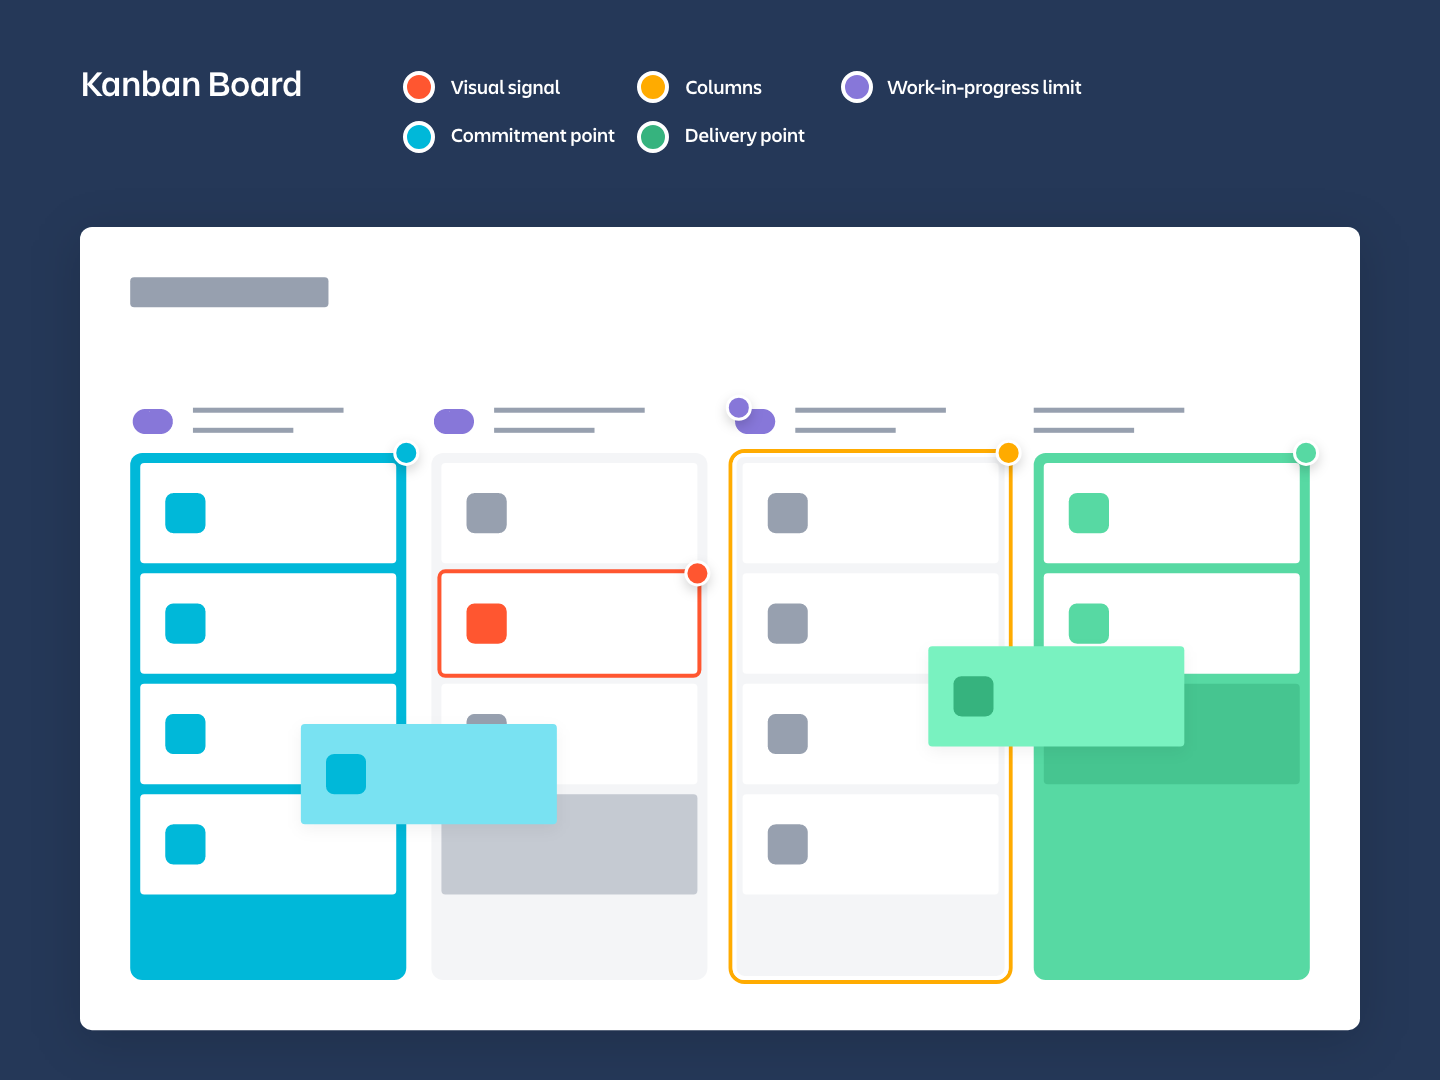
\includegraphics[scale=0.25]{img/obr4.png}
    \caption{Jednoduchá kanbasnká nástenka}
    \label{fig:kab-nas}
\end{figure}

\subsubsection{História}
\indent Trello bolo spustené v roku 2011 spoločnosťou Fog Creek. Za celou myšlienkou bol hlavne zakladateľ spoločnosti Joel Spolsky. Magazín Wired zaradil aplikáciu do „The 7 Coolest Startups You Haven´t Heard of Yet“ – Najlepších 7 startupov, o ktorých ste nepočuli. Tak isto sa v článku objavil názor, že Trello uľahčuje a svojim spôsobom spríjemňuje prácu na projektoch. 

\indent V máji 2016 ohlásilo Trello, že dosiahlo 1,1 milióna aktívnych používateľov denne a 14 miliónov celkovo založených účtov. V januári 2017 spoločnosť Atlassian kúpila Trello za 425 miliónov dolárov s tým, že 22\% podielu stále ostávala v rukách investorov a zakladateľa Joela Spolskeho. V roku 2019 nastal rapídny nárast používateľov kedy ešte v marci malo Trello 35 miliónov používateľov ale už v októbri to bolo 50 miliónov.
\subsubsection{Používateľské rozhranie}
\indent Prostredie aplikácie je veľmi jednoduché na používanie a nemá v sebe veľa zbytočných vecí. Tak isto navigácia v prostredí je veľmi jednoduchá a intuitívna. Registrácia je veľmi jednoduchá. Jediné čo nový používateľ potrebuje je meno, heslo a email. 

\indent Hneď po prihlásení sa používateľovi zobrazí nástenka kde vidí tímy, v ktorých je pridaný. Tak isto môže vytvoriť novú kartu tímu. Po vytvorení sa otvorí okno tímu, ktoré zväčša pozostáva z 3 stĺpcov – To Do, Doing a Done plus možnosť pridať ďalšie stĺpce. Tri dopredu vytvorené stĺpce sa samozrejme dajú vymazať alebo premenovať. 

\begin{figure}[H]
    \centering
    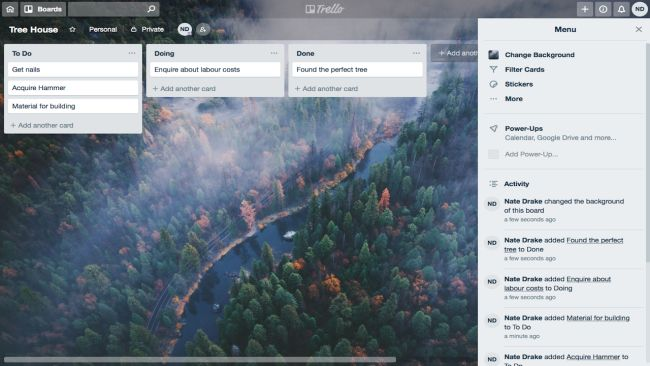
\includegraphics[scale=0.65]{img/obr-trello.jpg}
    \caption{Náhľad nástenky v aplikácii Trello}
    \label{fig:nastenka}
\end{figure}

\indent V jednotlivých stĺpcoch je potom možné vytvárať nové karty, ktoré reprezentujú nejakú úlohu, komunikáciu alebo čokoľvek čo tím potrebuje. Po kliknutí na kartu sa zobrazí okno kde sa nachádza popis karty, komentáre a možnosti čo sa dá s kartou robiť – priradiť kartu používateľom aby pri zmene na karte dostali upozornenie. Upozornenia sa dajú samozrejme aj vypnúť. Na jednotlivé nástenky je možné pridanie rôznych doplnkov ako je napríklad kalendár, Googke drive, Slack, Mapy alebo špecifické doplnky. 

\indent Po kliknutí na profil sa otvorí stránka používateľského profilu. Tu je možne zmeniť meno, pridať fotku profilu, zmeniť iniciály, zmeniť avatara z iniciálok na fotku, nastaviť politiku upozornení alebo pre farebne slepých používateľov je tu možnosť zapnutia módu pre farebne slepých. 

\begin{figure}[H]
    \centering
    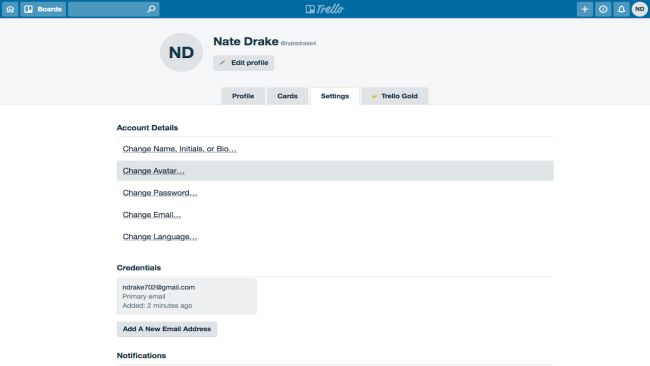
\includegraphics[scale=0.65]{img/obr-trello-profil.jpg}
    \caption{Stránka profilu v aplikácii Trello}
    \label{fig:profil}
\end{figure}

\subsubsection{Doplnky}
\indent Do jednotlivých násteniek alebo tímov sa dajú pridať rôzne doplnky, ktoré rozširujú možnosti použitia Trella. Okrem rôznych Botov, ktorí len posielajú preddefinované správy alebo upozornenia je ponuka doplnkov veľmi veľká – od štandardných doplnkov ako je kalendár, Dropbox, Google Drive, Slack, GitHub, až po špecifické určené nie len na co-working ako napríklad Card Family, Prize Checker, Prize Tag a iné. 
\subsubsection{Cena}
\indent Trello ponúka 3 typy účtov. Bezplatný, ktorý zahŕňa neobmedzený počet násteniek, kariet, členov tímu alebo príloh. Je možne pridať jeden doplnok na nástenku a je možné pridanie prílohy o veľkosti do 10MB alebo prepojiť akýkoľvek súbor z Google Drive, Dropbox alebo OneDrive účtu. 

\indent Business balík stojí 9,99\$ mesačne ale platí sa ročné predplatné. Balík ponúka to isté čo bezplatný balík s tým, že je možne pridať neobmedzený počet doplnkov na nástenku a je možné pridať 250MB prílohy. Ďalšími rozširujúcimi vecami je možnosť usporiadania násteniek do kolekcii, nastaviť kto tieto kolekcie môže vidieť alebo nahratie vlastných pozadí pre nástenky. 

\indent Enterprise balík stojí 20,83\$ mesačne pri ročnom predplatnom. Balík zahŕňa funkcionalitu Business balíka plus dvojfaktorová autentifikácia, šifrovanie súborov, vlastná kontrola zabezpečenia, vylepšené SLA. 

\subsection{Nedostatky aplikácii}
\indent Pri každej aplikácii okrem Facebook Workplace sme mohli vidieť, že využívajú rôzne doplnky. Pre použitie týchto doplnkov avšak musí používateľ zväčša disponovať účtom založeným v danej platforme. Napríklad ak chce používateľ v Slacku využívať Google kalendár musí mať založený účet na platforme Google. Táto skutočnosť je častokrát medzi používateľmi považovaná za otravnú a častokrát má používateľ potom zbytočne vytvorené účty na veľkom množstve platform, ktoré zvyknú používateľa aj spamovať na email. Preto do našej aplikácie chceme importovať služby, ktoré sú zväčša najžiadanejšie medzi službami ponúkanými doplnkami. 

\indent Druhým veľkým nedostatkom, ktorý by sme chceli našou aplikáciou odtrániť je nutnosť platenia. Je samozrejmé, že pre veľké firmy nie je problém si radšej priplatiť za stabilnú a 100\% funkčnú aplikáciu, ktorá poskytuje veľké množstvo služieb aj za cenu pridania veľkého množstva doplnkov. Avšak pre študentov je odstránenie potreby platenia za aplikáciu veľkým prínosom. Jedná sa hlavne o ostránenie limitu používateľov bez poplatku za aplikáciu. Pri niektorých aplikáciach je avšak poplatok aj za určité služby v podobe dopnkov. Toto sa v našej aplikácii tak isto nachádzať nebude. Každý používateľ bude mať plný a rovnaký prístup k aplikácii. Za základ našej aplikácie sme si zvolili rovnakú funkcionalitu ako má Slack bez doplnkov čiže vytvrenie tímov a komunikácia v nich. K tomu pridáme funkcionalitu doplnkov ako je kalendár s udalosťami, možnosť hlasovaní v tíme a jednoduchú nástenku úloh v tíme podobnú ako má Trello. 

\section{Možné technické problémy}
\indent Pri tvorbe akéhokoľvek softvéru sa vývojár stretne s množstvom situácii, ktoré môžu vyvolať pri používaní vyvýjaného softvéru problém. Preto musí vývojár už počas vyvýjania tohto softvéru tieto možné problémy odtrániť. V tejto kapitole sa preto budeme venovať možným technickým problémom, ktoré sa môžu vyskytnúť v našej pripravovanej aplikácii a načrtneme ako tieto problém plánujeme odstrániť.

\indent Preto aby sme správne identifikovali možné problémy si najskôr musíme ale povedať ako bude naša aplikácia vyvýjaná. Po zvážení sme sa rozhodli, že aplikácia bude vyvýjaná princípom web-aplikácie s tým, že bude mať na pozadí aj serverovú časť, ktorá bude zodpovedná za komunikáciu s databázou.

\subsection{Používateľské rozhranie}
\indent Pred pár rokmi pri vývoji web-aplikácii sa vývojár nemusel zamýšlať nad tým na akom zariadení bude používateľ spúšťať web-aplikáciu - smartfóny neexistovali a jediné zariadenie, na ktorom mohol používateľ otvoriť web-aplikáciu bol počitač cez prehliadač. Dnes avšak treba myslieť na to, že používateľ môže aplikáciu otvárať na smartfóne, tablete alebo inom zariadení. Preto musia byť web-aplikácie vyvýjané spôsobom aby sa zobrazovaná stránka vedela natívne prispôsobiť veľkosti obrazovky, na ktorej je zobrazovaná.

\indent Ďaľším faktorom je intuitívnosť využívania aplikácie. V dnešnej dobe sú v obľube jednoduché aplikácie, ktoré vie používateľ intuitívne používať. Či už sa jedná o prehľadnosť aplikácie alebo o navigáciu v aplikácii. Pokiaľ si využívanie aplikácie žiada najskôr si preštudovať dopodrobna ako aplikáciu používať, aplikácia stratí lojalitu používateľov. 

\indent Na odstránenie toho potencionálneho problému sme sa rozhodli našu aplikáciu vyvýjať v prostredi Ionic, ktoré nám umožňuje aplikáciu vyvýjať zároveň pre viac platform. V Ionicu je možné aplikáciu vyvýjať pre štandardný webový prehliadač, avšak zároveň je aplikácia vyvýjaná aj pre webové prehliadače v smartfónoch a tabletoch. Samozrejme je ale potrebné využívanie responzívných prvkov a elemtov aby sa vedeli automaticky prispôsobiť veľkosti obrazovky. Pred začatím vývoja sme sa ale dohodli web-aplikáciu po implementovaní vyexportovať pomocou framewrku Electron do štandarnej aplikácie pre platformu Windows. Pomocou Electronu je ale možné aplikáciu vyexportovať na akúkoľvek platfomu či už Linux, MacOS, Android alebo aj iOS len zmenou príkazu na exportovanie. Týmto by sa mal tento potencionálny problém s používateľským rozhraním odstrániť.

\subsection{Používateľské skúsenosti}
\indent Používateľia sa pri prechode na novú aplikáciu obávajú hlavne o to či ju budú vedieť používať. Preto v dnešnej dobe sa častokrát veľa aplikácii zameraných na určitú potrebu používateľa veľmi podobá. Je to hlavne preto aby používateľ mohol hneď s aplikáciou pracovať a nemusel sa učiť ako ju používať. Tento problém bol už čiatočne spomenutý pri probléme s používateľským rozhraním nakoľko je to s ním úzko späté. Na odstránenie tohto problému sme sa preto rozhodli vyvýjať našu aplikáciu tak aby bola podobná aplikácii Slack čo sa týka vyzuálnej stránky. Používateľ, ktorý používal už v minulosti aplikáciu Slack bude hneď vedieť ako využívať aj našu aplikáciu avšak tak isto bude design našej aplikácie prispôsobený tak aby ja používateľ, ktorý nevyužíval podobnú aplikáciu hneď vedel ako našu aplikáciu využívať.

\subsection{Výkon}
\indent Rýchlosť načítavania aplikácie a celková rýchlosť jednotlivých služieb, ktoré aplikácia ponúka je jedným z hlavných faktorov na prilákanie používateľov. Preto je potrebné aplikáciu vyvýjať tak aby jednotlivé služby neboli náročné na či už výpočtový čas alebo na hardvér zariadenia, na ktorom aplikácia beží. 

\indent Na ostránenie tohto problému bude preto potrebné aplikáciu implemenovať bez zbytočných chýb v kóde a písať kód čo najednoduchšie. Tak isto bude potrebné aby sme nevyužívali príliš náročné doplnky. Pri tomto probléme bude tiež potrebné dbať na rýchlosť načítavania a ukladania do databázy. Po preštudovaní viac potencionálne využiteľných databáz sme sa rozhodli využiť databázu CouchDB s replikovaním na lokálnu databázu PouchDB. Toto využitie dvoch databáz rozoberieme pri probléme so stratou pripojenia na internet.

\subsection{Strata pripojenia na internet}
\indent Tento problém môže nastať ktorémukoľvek používateľovi. Ake sme už vyžšie spomenuly naša aplikácia bude vyexportovaná ako desktopová aplikácia čiže spustiť bez pripojenia na internej ju pôjde avšak tu nastáva problém už pri prihlásení. Na prihlásenie bude potrebné byť pripojený na internet nakoľko sa prihlasovacie údaje musia overiť s online databázou. Potom avšak bude možné stratiť pripojenie na internet nakoľko využijeme replikáciu databázy na lokálnu databázu PouchDB. Táto databáza preberie všetky dáta pri prihláseni z online databázy a budeme môcť ich zobrazovať. Tak isto hneď pri akomkoľvek zápise je do online databázy je táto lokálne hneď aktualizovaná ak je teda zariadenie pripojené na internet. Ak pripojenie stratí bude zobrazovať len tie dáta, ktoré boli v databáze do straty pripojenia. 

\subsection{Bezpečnosť}
\indent Bezpočnosť dát, ktoré používateľ zadá na stránke je samozrejmosťou každej stránky. Je samozrejmé, že v tomto bode je dosť obtiažne zabrániť všetkým potencionálnym hrozbám. Tu je možné aj zvážiť, ktoré dáta sú dôležitejšie a ktoré menej. Za ochranu dát v databáze samozrejme zodpovedá čiastočne už aj samotný softvér použitej databázy ale treba zabezpečiť aj zariadenie, na ktorom databáza beži a dáta keď sú vytiahnuté z databázy a pracuje sa s nimi.

\indent V našej aplikácii sme sa hlavne zamýšľali na zabezpečením dát pri práci s nimi. Tu sme sa tiež rozhodovali, ktoré dáta bude treba zabezpečiť a ktoré nie. Tu sme za najdôležitejšie dáta zvolili prihlasovacie heslo používateľa. Ostatné dáta nie sú až také dôležité a aj s prihliadnutím na náročnosť aplikácie sme sa rozhdoli zabezpečiť len heslo. Heslo bude hneď pri registrácii na strane servera zašifrované pomocou prídavnej knižice do node.js bcrypt a tak uložené do databázy. Po zašifrovaní už heslo nikdy nebude rozšifrovávané čiže pri prihlasovaní sa zadané heslo pomocou funkcie knižnice bcrypt overí so zašifrovaným heslom a na základe toho bude overená správnosť zadaného hesla. 

\indent Zabezpečovanie servera nebudeme relaizovať keďže aplikácia bude testovaná len na lokálnom stroji. Ak by sa ďalej uvažovalo o distribúciu aplikácie bude samozrejme možné zabezpečenie servera ako aj samotnej aplikácie rozšíriť.

\subsection{Zhrnutie}
\indent Tieto problémy sú asi najzásadnejšie a najväčšie, s ktorými sa stretneme pri vývoji aplikácie. Jendým menej zásadným problémom, ktorý ale ešte stojí za zmienku je problém možnosti rozšírenia aplikácie. Niektoré aplikácie sú implementované tak, že je skoro nemožné k nim po vydaní dorobiť nejaké rozšírenie alebo dodatok. Pri implementovaní našej aplikácie na to budeme myslieť a bude implementovaná tak aby sa k nej jednoducho dala dorobiť ďaľšia funkcionalita.

\section{Použité technológie}
\indent V nasledujúcej kapitole zhrnieme technológie, ktoré sme sa rozhodli použiť na implemtovanie našej aplikácie. Ku každej technológii popíšeme možnosti, ktoré plánujeme využiť nakoľko rozpísať všetky možnosti je pre nás zbytočné.

\subsection{Node.js}
\indent Node.js je na svojich stránkach popísaný ako JavaScript zameraný na udalosti pre tvorbu škálovateľných sieťových aplikácii. Na nasledovnom príklade jednoduchej aplikácie Hello World môžeme vidieť, že sa mnoho spojení dá zvládnuť súčasne - Obr.~\ref{fig:node_hello}. Po každom spojení sa spustí spätné volanie - callback, ale ak nie je potrebné vykonať žiadnu akciu program bude spať kým ho niekto nezavolá. 

\begin{figure}[H]
    \centering
    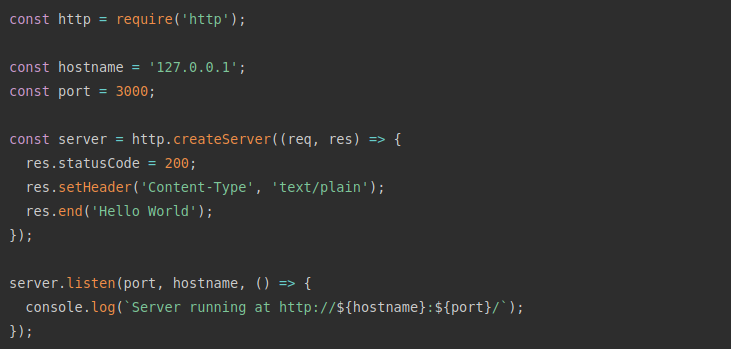
\includegraphics[scale=0.55]{img/node_hello.png}
    \caption{Jednoduchý program Hello World v Node.js}
    \label{fig:node_hello}
\end{figure}

\indent Toto je v rozpore s dnešným bežnejším a modernejším prístupom založeným na vláknach operačného systému, ktoré bežia súčasne. Vytváranie vlákien pri sieťovej komunikácii je relatívne neefektívne a veľmi náročné na používanie. Mimo toho sú používatelia servera Node.js bez obáv takzvaného mŕtveho zablokovania procesu, pretože neexistujú žiadne zámky. Takmer žiadna akcia v Node.js priamo nevykonáva I/O, takže proces sa nikdy neblokuje. Preto sa odporúča na škálovateľné aplikácie používať Node.js.

\subsubsection{História}
\indent Node.js bol vytvorený Ryanom Dahlom v roku 2009 a bol podporovaný len pre platformy Linux a MacOS. Pre porovanie prvé prostredie pre JavaScript na strane servera LiveWire Pro Web bolo uvedené na trh v roku 1996. Údržba a ďaľší vývoj bol najskôr vedený len samotným Dahlom, ale neskôr bol sponzorovaný firmou Joyent. Dahl prezentoval Node.js 8. Novembra 2009 na konferencii European JSConf. Node sa vtedy skadal z JavaScriptovehé enginu V8 od spoločnosti Google, udalostnej slučky (event loop) a nízko-úrovňového I/O API.

\indent V januári 2010 prišiel na trh NPM - správca balíkov pre Node.js. Tento správca umožňuje používateľom Node.js zdielanie a publikovanie zdrojové kódy doplnkových modulov. Zároveň uľahčuje ich sťahovanie, inštaláciu a aktualizáciu. Neskôr v lete 2011 Microsoft a Joyent spolupracovali na vytvorení podpori Node.js pre Windows, ktorú v tom roku aj vydali. 

\indent V roku 2014 po nezhodách pri vývoji sa časť komunity odštiepila a vytvorila io.js. O rok neskôr vznikla, ale Node.js Foundation, ktorá zjednotila roztrieštenú komunitu a zjednotila Node.js v0.12 a io.js v3.3 do Node v4.0. Toto zjednotenie prinieslo novinky z ES6 z V8 a zároveň umožnila dlhodobo trvajúci vývoj platformy.

\subsubsection{Architektúra Node.js}
\indent Každá platforma má svoju architektúru, tak isto aj Node.js. V tejto kapitole rozoberieme jej hlavné vlastnosti a časti. Nie všetky budeme potrebovať pri implementácii ale je dobré ich poznať.

\indent Základnou vlastnosťou je, že Node.js má asynchrónne a udalostne riadené API. Toto zaručuje to, že nasledujúce volania nie sú blokované predchádzajúcim volaním. V praxi to znamená, že Node.js nikdy nečaká kým je z volania vrátená hodnota respektíve je volanie dokončené a ukončené. Server sa po zavolaní volania presunie na ďaľšie a vnútorný notifikačný mechanizmus udalosti dostane odpoveď z prechádzajúcich volaní vtedy keď sú dokončené a dostane sa tým aj k výsledku. 

\indent Druhou veľkou výhodou je existencia udalostnej slučky. Vďaka tomu je jednovláknový a vysoko škálovateľný. Vyžšie spomínaný udalostný mechanizmus napomáha serveru vrátiť odpoveď bez blokovania. Tým sa server stáva vysoko škálovateľný v porovnaní s tradičnými riešeniami na strane servera, ktoré majú obmedzený počet vlákien a tým sa aj počet požiadaviek, ktoré sú spracované súčasne stáva obmedzený. 

\indent Ďaľšou výhodou je, že aplikácie založené na platforme Node.js sú bez vyrovnávacej pamäte, číže údaje posielané na výstup sú zoskupované do malých blokov.

\indent Na Obr.~\ref{fig:node_arch} môžeme vidieť základné rozdelenie architektúry platformy Node.js. 

\begin{figure}[H]
    \centering
    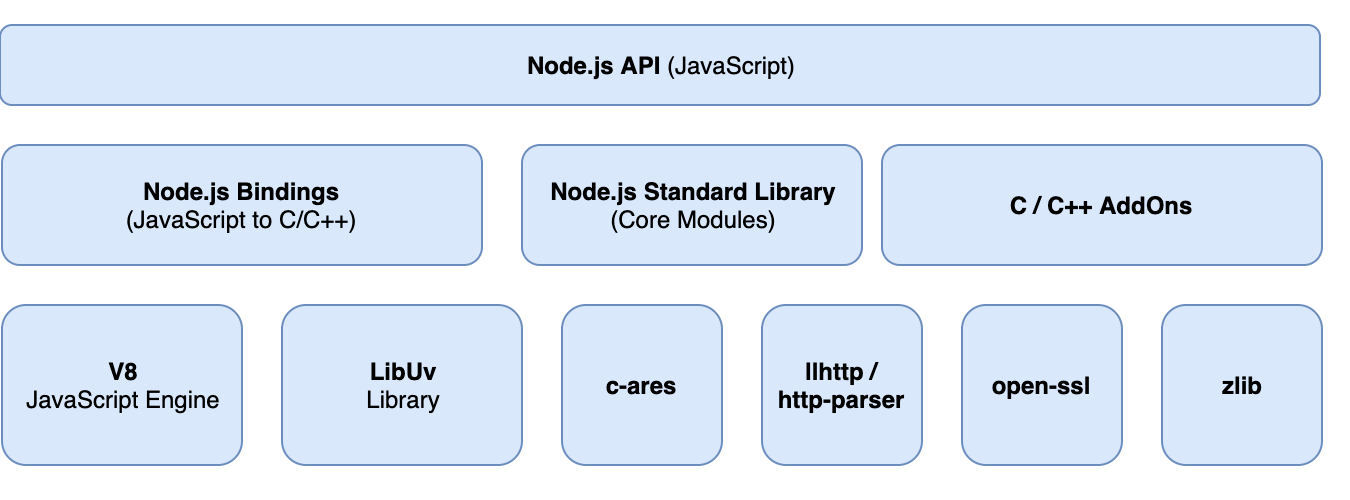
\includegraphics[scale=0.30]{img/node_architecture.png}
    \caption{Architektúra platformy Node.js}
    \label{fig:node_arch}
\end{figure}

\indent Na vrchole sa nachádza Node.js API, ktoré je napísané v JavaScripte a je možné k nemu priamo pristupovať za účelom využitia v aplikáciach. Pod API sa nachádza trio Node.js Bindings, Node.js Standard Libraries a C/C++ AddOns. Node.js Standard Libraries sú funkcie súvisiace s knižnicami operačného systému a umožňujú využívanie napríklad časovačov, súborového systému alebo sieťových volaní http. Node.js Bindings je knižnica, ktorá umožňuje komunikáciu JavaScriptu s C/C++ a tým ich viaže dokopy. Poslednou časťou sú C/C++ AddOns čo sú dynamicky linkované doplnky viazané na C/C++ knižnice. Toto umožňuje vytvorenie akejkoľvek C/C++ knižnice a jej využitie v Node.js. 

\indent Na spodku sa náchádzajú knižnice C/C++:
\begin{itemize}
    \item V8 JavaScript Engine - konvertuje JavaScript do strojového kódu daného operačného systému
    \item LibUv - multiplatformová C knižnica zameriavajúca sa na asynchrónne I/O operácie
    \item c-ares - C knižnica pre asynchrónne DNS požiadavky a odpovede
    \item http-parser - C knižnica pre HTTP požiadavky a odpovede
    \item open-ssl - kryptografické funkcie
    \item zlib - C knižnica pre synchrónnu aj asynchrónnu kompresiu, dekompresiu a pre streamovanie dát 
\end{itemize}

\subsubsection{Event loop}
\indent Event loop alebo udalostná slučka je to čo umožnuje Node.js vykonávať neblokujúce vstupno-výstupné operácie napriek tomu, že JavaScript je jednovláknový. Keďže väčšina moderných jadier má viacvláknové spracovanie tak môžu zvládnuť vykonávať viac operácii na pozadí. V Node.js to ale funguje tak, že keď je jedna z operácii dokončená, jadro povie Node.js, aby do fronty na vykonanie pridalo príslušné spätné volanie na výsledok vykonanej operácie. Na Obr.~\ref{fig:event_loop} môžeme vidieť zjednodušený diagram ako to funguje. 

\begin{figure}[H]
    \centering
    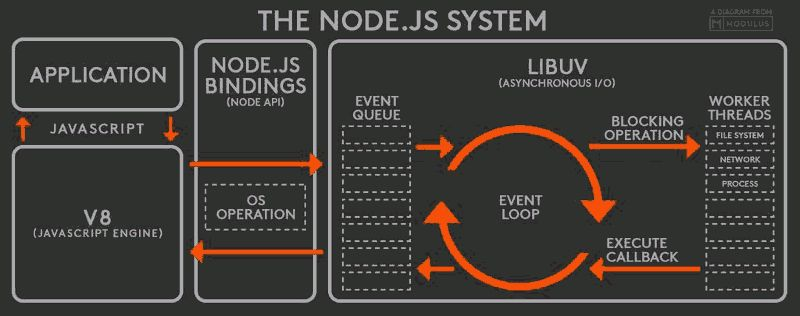
\includegraphics[scale=0.55]{img/evet_loop.jpg}
    \caption{Zjednodušená verzia fungovania Node.js architektúri}
    \label{fig:event_loop}
\end{figure}

\indent Keď sa Node.js spustí tak inicializuje slučku udalostí a spustí poskytnutý vstupný skript, ktorý môže uskutočňovať asynchrónne volania API. Následne sa začne spracovávať slučka udalostí. Tá postupne spracováva udalosti z fronty udalostí bez toho aby čakala na dokončenie daných udalostí. Keď je táto udalost hotová tak sa jej spätné volanie zaradi na spodok fronty udalostí a jej výsledok je teda znova spracvaný keď sa k nemu slučka dostane. Toto sa opakuje kým nie je fronta udalostí vyčerpaná alebo nie je dosiahnutý maximálny počet spätných volaní. 

\subsubsection{Nevýhody Node.js}
\indent Ako sme vyžšie popísali Node.js má veľké množstvo výhod, medzo ktoré hlavne patrí asynchrónne I/O, škalovateľnosť, veľká a aktívna komunita a veľke množstvo prídavných modulou. Avšak Node.js má aj určité nevýhody. Medzi hlavné patrí:
\begin{itemize}
    \item neefektívnosť pri náročných procesoch pre CPU - tvorba reportov, analýz, zložité výpočty... 
    \item pri nepochopený práce s callbackmi môže viesť používanie Node.js k zle napísaným kódom
    \item menej štandarných knižníc v porovnaní s klasickou Javou a .NET platformou
\end{itemize}

\indent Môžeme teda vidieť, že nie vždy je využitie Node.js možnosťou. Veľmi záleží akú aplikáciu vyvíjame. Ak pracujeme na aplikácii pre real-time komunikáciu s využitím websockeov, streaming alebo rýchlu prácu so súbormi tak je Node.js veľmi vhodný. 

\subsection{Node Package Manager}
\indent Node package manager, skrátene len NPM je správca prídavných balíkov vyvinutý pre Node.js. Oficiálna stránka \textit{https://www.npmjs.com} obsahuje tisícky voľných balíkov na stiahnutie a používanie. NPM program sa automaticky naištaluje pri inštalácii Node.js. NPM sa následne dá spúšťat z príkazového riadku. Tak isto je možné vytvorenie vlastného balíka a nahratie ho do centrálneho repozitára oficiálnej stránky NPM.

\indent Balík v Node.js je zväčša adresár obsahujúci všetky súbory, ktoré pridavný modul potrebuje. Modul je JavaScriptová knižnica, ktorú programátor môže pridať do svojho projektu. Jedným zo súborov, ktoré sa nachádzajú v adresári musí byť metadátový súbor s názvom \textit{package.json}. V tomto súbore sú definové vlastnosti, meno a verzia balíka. Na Obr.~\ref{fig:package} môžeme vidieť ako takýto súbor vyzerá.  

\begin{figure}[H]
    \centering
    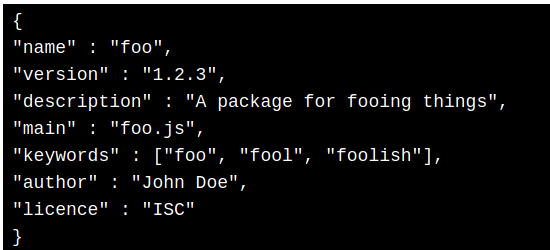
\includegraphics[scale=0.55]{img/package.png}
    \caption{Jednoduchý \textit{package.json} súbor}
    \label{fig:package}
\end{figure}

Inštalácia balíkov sa dá zrealizovať tromi spôsobmi:
\begin{itemize}
    \item manuálna inštalácia len pre projekt, na ktorom pracujeme - v termináli sa v priečinku projektu zavolá príkaz \textbf{npm instal \textit{názov\char`_modulu}}. Posledná verzia balíka sa nainštaluje pre projekt a uloží do adresára \textit{node\char`_modules}.
    \item manuálna inštalácia globálne pre systém - v termináli sa zavolá príkaz \textbf{npm instal \textit{názov\char`_modulu} -g}. Táto možnosť sa ale neodporúča.
    \item poslednou možnosťou je dopísanie do projektového suború \textit{package.json} do časti dependencies názov modulu a jeho verziu a v termináli zadať príkaz \textbf{npm install}.
\end{itemize}

\section{Návrh aplikácie}
\indent Témou diplomovej práce je implemetovať co-working aplikáciu s využitím webového frameworku Ionic/Angular s neskorším exportom na desktopovú aplikáciu pomocou Electronu na strane frontendu a s použitím Node.js a CouchDB na strane servera. V tejto kapitole sa budeme zaoberať návrhom celej aplikácie s využitím daných technológii na jednotlivých komponentoch. 

\begin{figure}[H]
    \centering
    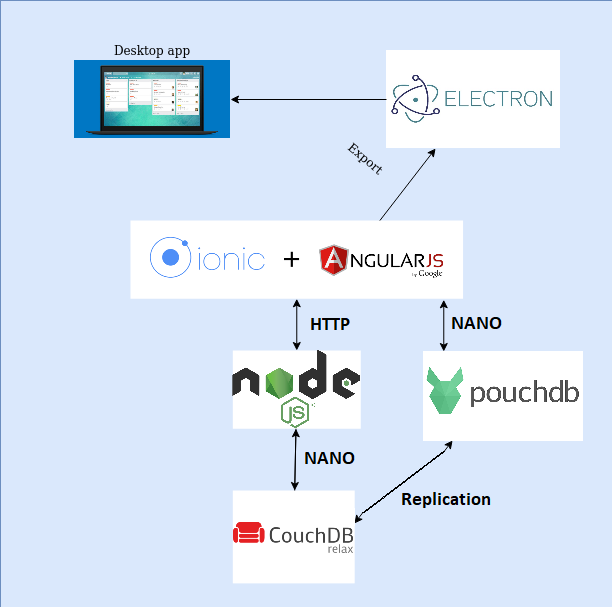
\includegraphics[scale=0.60]{img/diagram.png}
    \caption{Návrh komunikácie medzi komponentami}
    \label{fig:diagram}
\end{figure}

\indent Po prieskume aktuálnych technológii sme sa rozhodli využiť Node.js ako náš server, ktorý bude komunikovať s našou NoSql databázou CouchDB, do ktorej bude ukladať zadané dáta a zároveň posielať žiadané dáta na frontend implementovaný pomocou typescriptovo založeného frameworku Ionic. Ionic sa avšak ako bolo spomenuté v kapitole .... využíva na tvorbu webových alebo mobilných aplikácii. Preto finálnu webovú aplikáciu exportujeme nakoniec pomocou Electronu na desktopovú aplikáciu pre platformu Windows/Linux/MacOS.

\subsection{Špecifikácia požiadaviek}
\indent Prvým krokom pri tvorbe návrhu je špecifikovanie vlastností a celkového správania aplikácie. Definuje sa tu funkcionalita, ktorú chceme aby naša aplikácia mala, správanie aplikácie v určitých situáciách a jej kľúčové parametre, ktoré musí podľa požiadaviek spĺňať.
\subsubsection{Používateľské požiadavky} 
\indent Používateľské požiadavky sa stanovili na základe prehľadu co-working aplikácii, ktoré už existujú. Za základ sa zobrali hlavné funkcionality Slacku a k nim sa pridali buď doplnky Slacku alebo funkcie iných aplikácii. Softvér bude mať 2 používateľské rozhrania kedy jedno bude slúžiť ako administrátorské určené pre vedúcich tímov a klasické prostredie určené pre členov tímu. Administrátorské konto bude mať možnosť sa medzi týmito dvoma prostrediami prepínať. Administrátorské prostredie bude umožňovať vytváranie tímov, pozívanie a pridávanie členov tímu a manažovanie taskov. Prostredie člena tímu bude umožňovať vytváranie miestností na stránke tímu, vytváranie stretnutí, zahajovanie hlasovaní, pridávanie príspevkov do miestností, komentovanie príspevkov, komunikáciu medzi členmi tímu, pridanie kontaktu, akceptovanie alebo zamietnutie pozvánky do tímu, správu svojich taskov.

\textbf{Funkcionálne požiadavky:}

\underline{\textit{Administrátor:}}
\indent\begin{itemize}
    \item Prihlásenie a odhlásenie
    \item Vytvorenie tímu
    \item Pridanie používateľa do tímu
    \item Vytvorenie tasku
    \item Pridanie používateľa do tasku
    \item Nastavenie stavu tasku
    \item Prepnutie sa medzi rozhraniami aministrátor a používateľ
\end{itemize}


\underline{\textit{Člen tímu:}}
\indent\begin{itemize}
    \item Prihlásenie a odhlásenie
    \item Akceptovanie pozvánky do tímu
    \item Pridanie miestnosti v tíme a nastavenie či bude verejná alebo súkromná
    \item Pridanie ľudí do miestnosti ak je súkromná
    \item Pridanie udalosti v tíme
    \item Spravovanie svojich taskov
    \item Zahájenie hlasovania
    \item Pridanie kontaktu do svojho zoznamu kontaktov
    \item Nápisanie správy inému používateľovi
    \item Komentovanie príspevkov v miestnosti
    \item Prezeranie svojho kalendára\newline
\end{itemize}


\textbf{Nefunkcionálne požiadavky:}
\indent\begin{itemize}
    \item Používateľsky prijateľné prostredie
    \item Obsluha viacerých používateľov
    \item Používateľské rozhranie implementované prostredníctvom desktopovej aplikácie
    \item Dizajn inšpirovaný aplikáciou Slack
\end{itemize}

\subsection{Diagramy}
\indent Po zadefinovaní požiadaviek môžeme pristúpiť k ďalšej časti, z ktorej návrh aplikácie pozostáva a to k diagramom. Podľa týchto diagramov sa potom pri implementácii budeme riadiť nakoľko tie nám presne ukazujú ako sa bude systém správať pri používaní a ako majú jednotlivé komponenti a časti aplikácie medzi sebou komunikovať. Základným diagramom, ktorý si vytvoríme ako prvý bude diagram prípadov použitia, ktorý nám buďe ukazovať ako jednotlivý herci - typy používateľov môžu používať aplikáciu. Ďalej existujú diagramy tried, ktoré pomáhajú vývojárovi vizualozovať si jednotlivé triedy, ktoré sa tvoria pri objektovo oriantovaných jazykoch. V našom prípade ale tento diagram vytvárať nebudme nakoľko nami používaný JavaScript ani TypeScript nie sú klasické objektovo oriantované jazyky. Diagramy, ktoré ale budeme určite vytvárať sú sekvenčné. Tie nám vizualizujú interakciu medzi komponentami alebo časťami kódu v aplikácii.

\subsubsection{Diagramy prípadov použitia}
\indent Diagramy prípadov použitia sa používajú na popísanie správania systému z hľadiska jeho používania. Ukazujú aký rôzny používatelia môžu systém používať a aké činnosti môžu v tomto systéme vykonávať.

\indent Obrázok~\ref{fig:use_case_pozivatel} nám ukazuje základné možnosti akéhokoľvek používateľa nášho systému. Tento používateľ sa najskôr musi registrovať do systému. Potom sa môže prihlásiť. Po prihlásení má na výber pod akým typom používateľa sa chce aktuálne prihlásiť - či pod administrátorom alebo ako člen tímu. 

\begin{figure}[H]
    \centering
    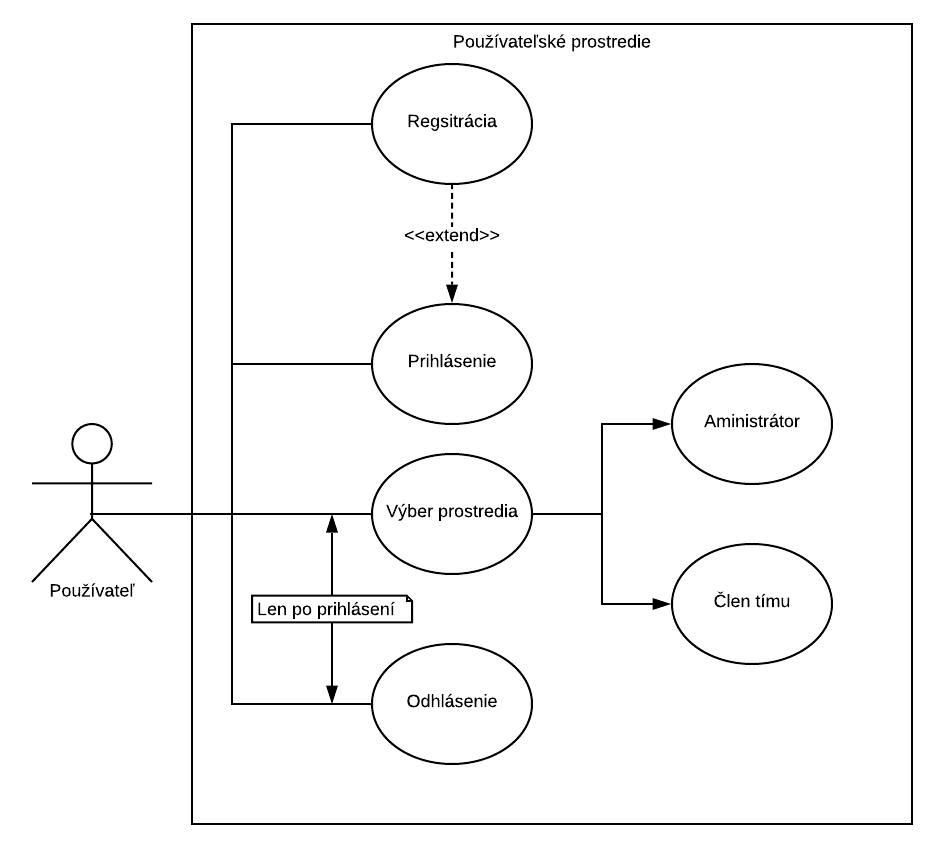
\includegraphics[scale=0.50]{img/DP_use_case_pouzivatel.png}
    \caption{Use case diagram pre používateľské prostredie}
    \label{fig:use_case_pozivatel}
\end{figure}

\indent Druhý diagram - Obr.~\ref{fig:use_case_administrator} nám ilustruje prípady použitia ak používateľ vybral možnosť prihlásiť sa ako administrátor prípadne ak sa člen tímu prepol do admnistrátorského rozhrania. Administrátor teraz môže buť spravovať svoje tími alebo vytvoriť nový tím.

\begin{figure}[H]
    \centering
    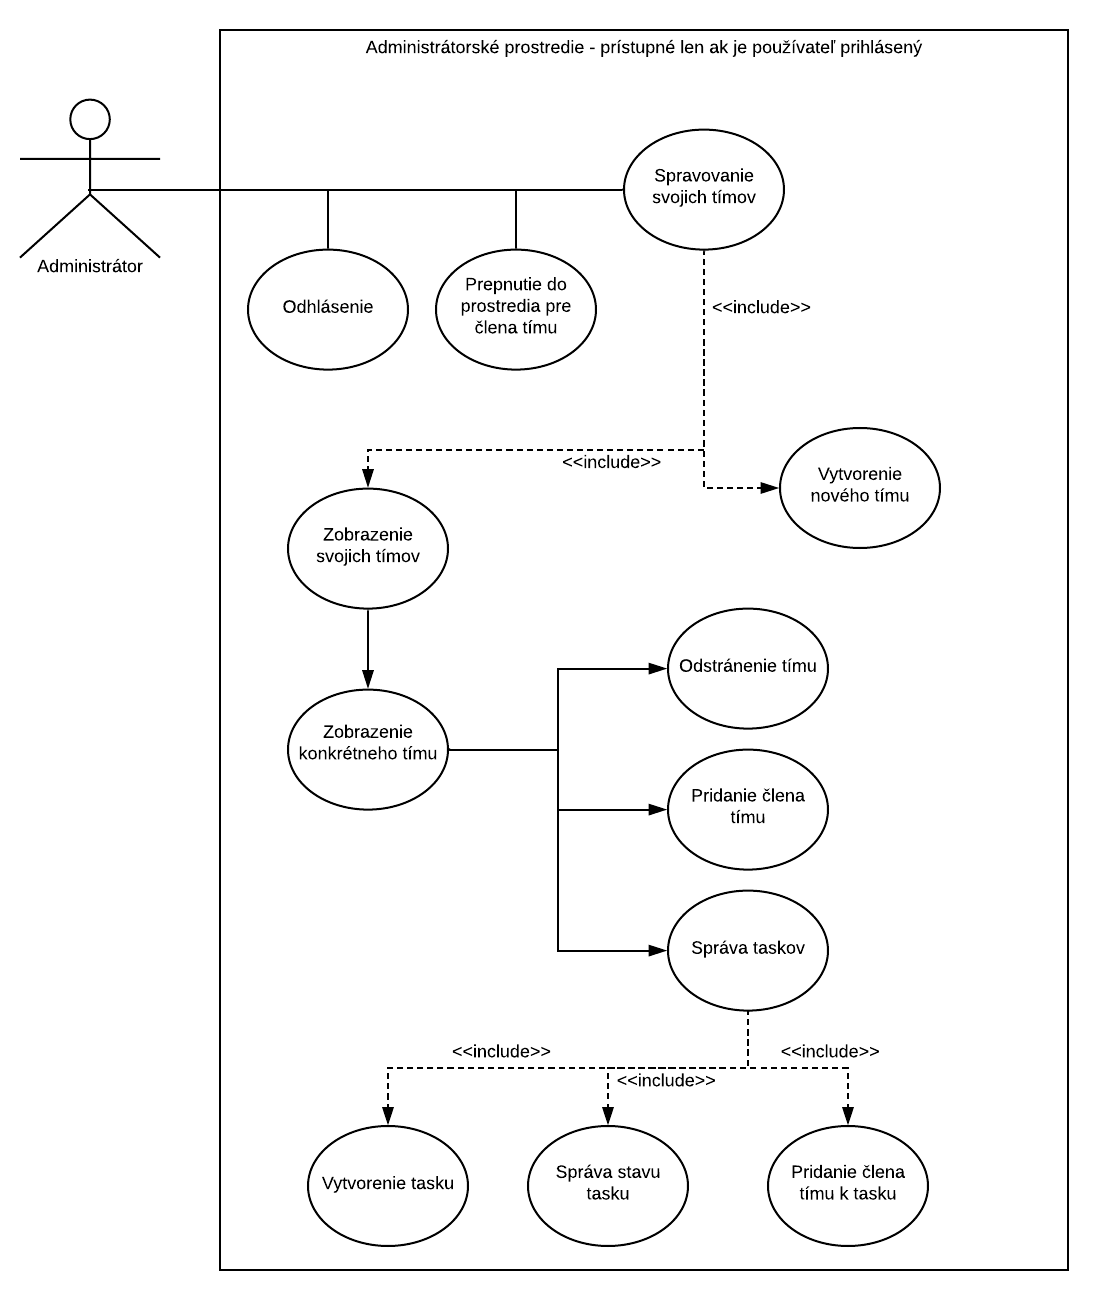
\includegraphics[scale=0.45]{img/DP_use_case_administrator.png}
    \caption{Use case diagram pre administrátorské prostredie}
    \label{fig:use_case_administrator}
\end{figure}

\indent Posledný diagram prípadov použitia - Obr.~\ref{fig:use_case_clen_timu} nám ilustruje ako môže používateľ používať systém ak si vybral možnosť prihlásiť sa ako člen tímu alebo sa prepol z admnistrátorského rozhrania do rozhrania člena tímu. Tu má používateľ na výber viacero možností čo môže v aplikácii vykonať.

\begin{figure}[H]
    \centering
    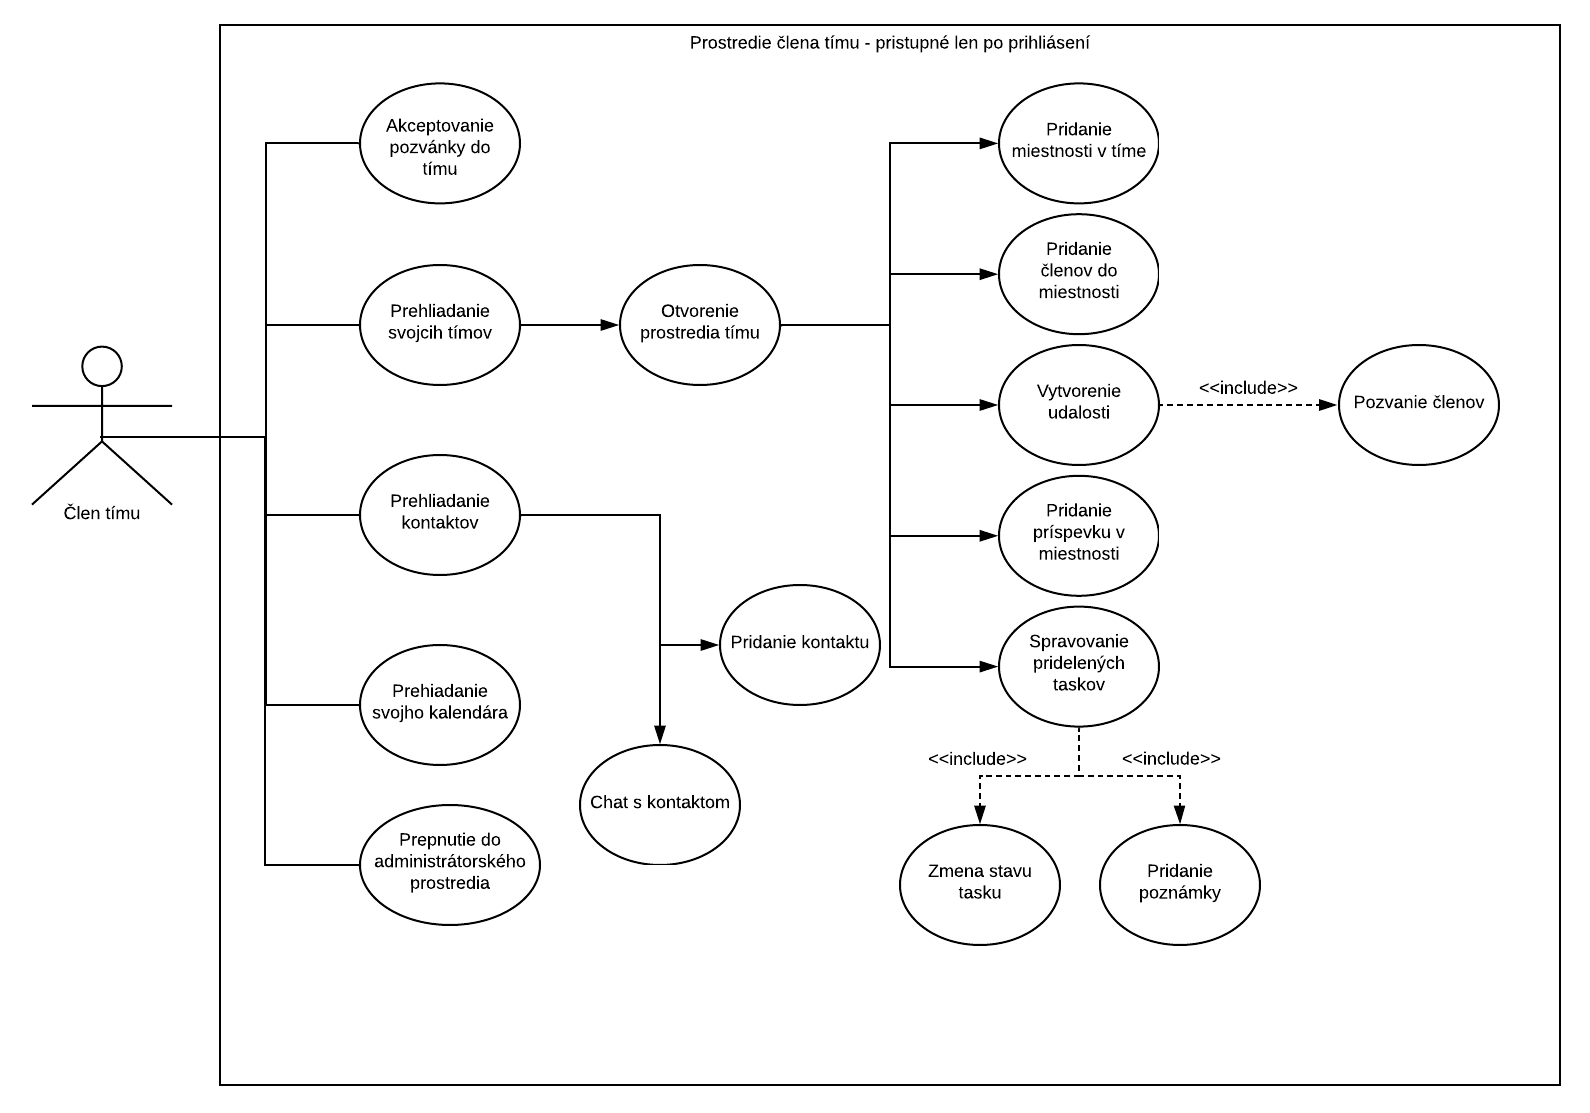
\includegraphics[scale=0.45]{img/DP_use_case_clen_timu.png}
    \caption{Use case diagram prostredia člena tímu}
    \label{fig:use_case_clen_timu}
\end{figure}

\subsubsection{Sekvenčné diagramy}
\indent Nasledujúce diagramy budú asi najpoužívanejšie pri implemtácii aplikácie nakoľko sekvenčné diagramy nám ukazujú interakcie medzi komponentami v systéme.
\newline
\newline
\textbf{Prihlásenie a registrácia} \newline
\indent Na Obr.~\ref{fig:seq_login} môžeme vidieť komunikáciu jednotlivých komponentov pri prihlásení alebo registrácii do aplikácie. Na základe výberu používateľa či sa chce prihlásiť alebo registrovať sa mu zobrazí príslušná stránka. Pri prihláseni sa po vyplnení údajov, tieto údaje pošlú na server, ktorý v online databáze skontroluje daný email či používateľ extistuje. Ak existuje skontroluje aj heslo. Ak sú oba údaje správne, server vytvorí autorizačný token s určitou platnosťou a pošle ho kientovi. Na strane klienta sa potom vytvorí lokálna databáza, ktorá si hneď z online databázy stiahne všetky dáta a aplikáciu tu začína pracovať len s lokálnou databázou. 

\begin{figure}[H]
    \centering
    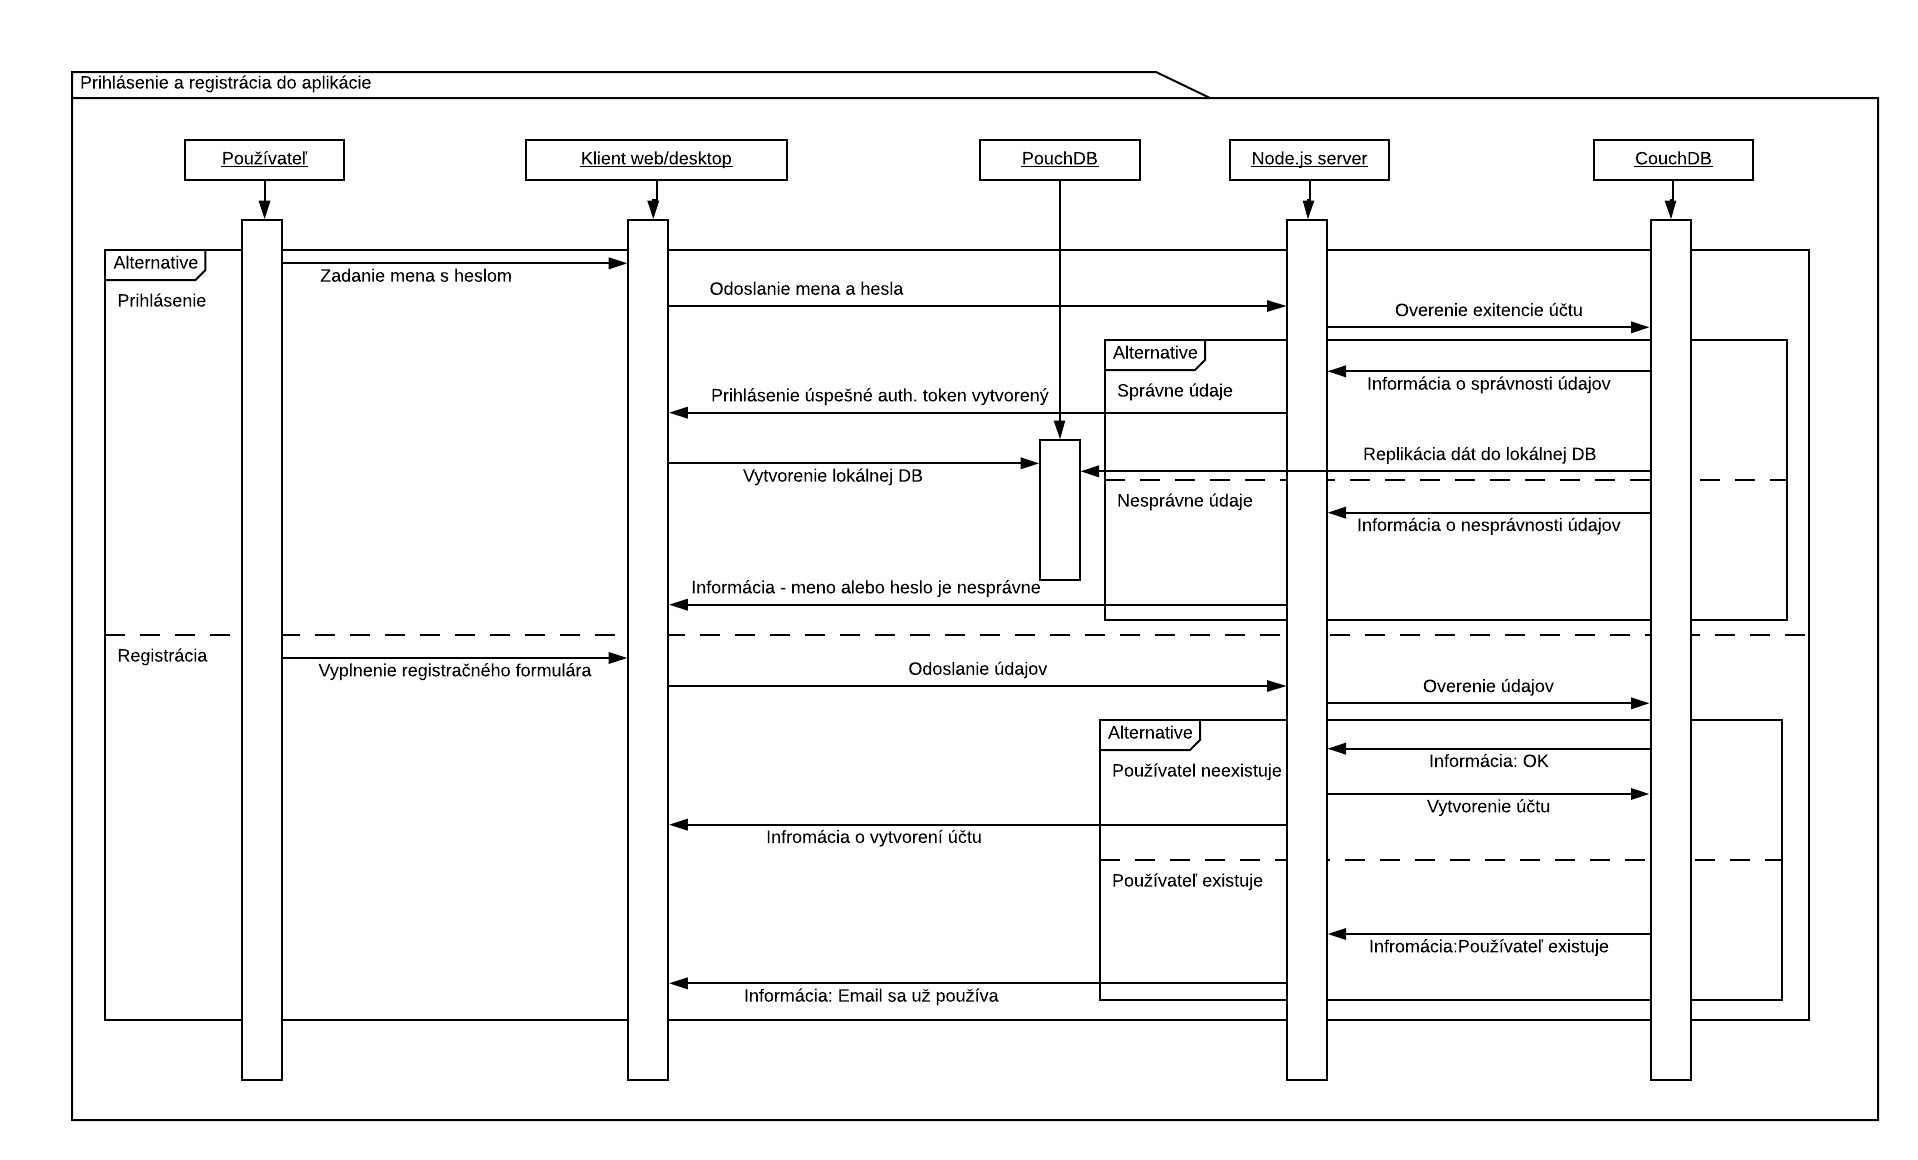
\includegraphics[scale=0.50]{img/Seq_login_register.png}
    \caption{Sekvenčný diagram prihlásenia a registrácie}
    \label{fig:seq_login}
\end{figure}

\indent Pri registrácii funguje systém podobne. Po vyplnení údajov sa údaje pošlú na server, ktorý overí či daný email sa auž nepoužíva. Ak sa nepoužíva tak sa do databázy uloží nový používateľ a na stranu klienta je odoslaná správa o úspešenej registrácii. 
\newpage
\textbf{Komunikácia komponentov v aplikácii po prihlásení} \newline
\indent Diagram Obr.~\ref{fig:seq_com} nám znázorňuje ako budú jednotlivé komponenty v aplikácii medzi sebou komunikovať po prihlásení do aplikácie.
\begin{figure}[H]
    \centering
    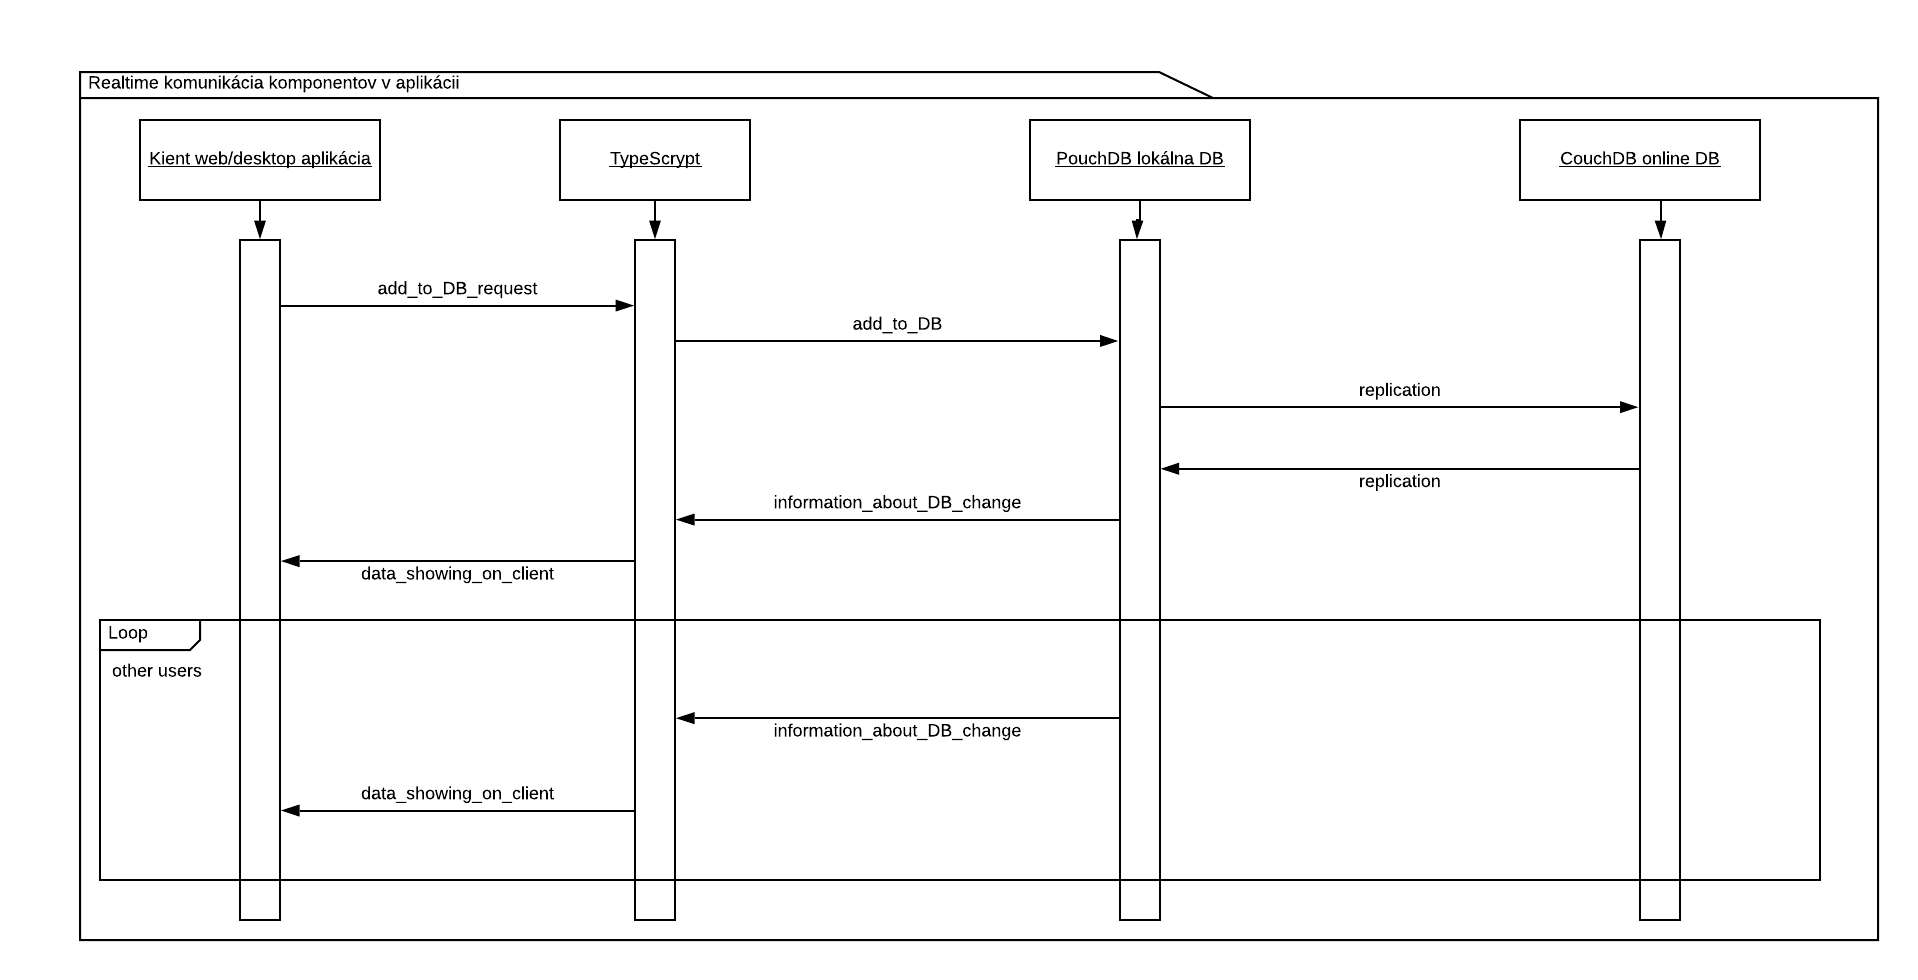
\includegraphics[scale=0.50]{img/seq_tim.png}
    \caption{Sekvenčný diagram komunikácie komponentov v aplikácii}
    \label{fig:seq_com}
\end{figure}

\indent Celá komunikácia je založená na http protokole. Na diagrame môžeme vidieť, že ak niektorý používateľ vytvorí tím, udalosť, úlohu alebo napíše správu tak je vytvorená žiadosť na pridanie do databázy. Pridanie do databázy je realizované tak, že najskôr sú dáta pridané do lokálnej databázy PouchDB a ak má zariadenie, na ktorom beží aplikácia prístup na internet sú teito dáta hneď zreplikované do online databázy. Ak prístup na internet nie je tak sú dáta zatial uložené len v lokálnej databáze do doby kým zariadenie nezíska prístup na internet. Ostatným používateľom je potom odoslaná infromácia, že na strane databázy prišlo k zmene a ich dáta, ktoré sa v klientovi zobrazujú sú aktualizované na základe nových dát v databáze.  

\subsection{Databázový model CouchDB}
\indent Po analýze viacrých možností sme sa v našom zadaní rozhodli nepoužiť štandardnú SQL databázu. Toto má za následok to, že sa nedá modelovať databáza cez štandarné ERD diagramy. CouchDB je databáza založené nie na tabuľkách ale na JSON dokumentoch. Hoci si naša aplikácia bude vyžadovať viac špecifických objektov pre jednotlivé záznamy do databázy, tieto objekty nebudú zložité. Jedná sa prevažne o objekty zložené z viacerých jednoduchým dátových hodnôt typu string, integer, date. Tieto objekty bude potrebné vytvoriť ako na strane servera v JavaScripte tak aj na strane frontendu v TypeScripte. Model potrebných objektov môžeme vydieť na naledujúcom obrázku- Obr. 

WorkVersion

\textbf{User:}
\indent\begin{itemize}
    \item základné údaje meno priezvisko heslo mail
    \item kontakty - pole id userov z DB
    \item workspace - pole id miestnosti z DB
    \item kalendar - pole id udalosti z DB
\end{itemize}

\textbf{Udalost:}
\indent\begin{itemize}
    \item nazov
    \item tím - id timu v ktorom udalost je
    \item zaciatok
    \item koniec
    \item ucastnici - pole id userov z DB
\end{itemize}

\textbf{Tím:}
\indent\begin{itemize}
    \item nazov
    \item admin - id usera z DB
    \item clenovia - pole id userov z DB 
    \item miestnosti - pole id miestnosti z DB
    \item udalosti - pole id udalosti z DB 
    \item tasky - pole id taskov patriacich timu
\end{itemize}

\textbf{Miestnost:}
\indent\begin{itemize}
    \item nazov
    \item typ - true=sukromna, false=verejna
    \item clenovia - pole id userov z DB - ak verejna automaticky prida vsetkych clenov timu
    \item prispevok - pole id prispevkov z DB
    \item hlasovania - id z DB aktualneho hlasovania
\end{itemize}

\textbf{Prispevok:}
\indent\begin{itemize}
    \item text
    \item autor - id usera z DB
    \item cas pridania
    \item komentare - pole id komentarov z DB
\end{itemize}

\textbf{Komentar:}
\indent\begin{itemize}
    \item text
    \item autor - id usera z DB
    \item cas pridania
\end{itemize}

\textbf{Sprava:}
\indent\begin{itemize}
    \item text
    \item autor - id usera z DB
    \item komu - id usera z DB
    \item cas odoslania
\end{itemize}

\textbf{Hlasovanie:}
\indent\begin{itemize}
    \item text
    \item autor - id usera z DB
    \item tim
    \item miestnost
    \item prva moznost
    \item druha moznost
    \item pocet za prvu
    \item pocet za druhu
\end{itemize}

\textbf{Task:}
\indent\begin{itemize}
    \item text
    \item tim
    \item prideleni useri - pole id userov z DB
    \item stav tasku
    \item poznamky - pole id komentarov z DB
\end{itemize}

\indent Obrazky ... - ... \textbf{Doplni sa ked bude DB hotová s pár dátami} sú záznamy jednotlivých objektov z CouchDB kde môžeme vidieť aj jednotlivé typy záznamov. 
